% !TEX encoding = UTF-8 Unicode

% Format teze zasnovan je na paketu memoir
% http://tug.ctan.org/macros/latex/contrib/memoir/memman.pdf ili
% http://texdoc.net/texmf-dist/doc/latex/memoir/memman.pdf
% 
% Prilikom zadavanja klase memoir, navedenim opcijama se podešava 
% veličina slova (12pt) i jednostrano štampanje (oneside).
% Ove parametre možete menjati samo ako pravite nezvanične verzije
% mastera za privatnu upotrebu (na primer, u b5 varijanti ima smisla 
% smanjiti 
\documentclass[12pt,oneside]{memoir} 

% Paket koji definiše sve specifičnosti master rada Matematičkog fakulteta
\usepackage[latinica]{matfmaster} 
%

\usepackage{amsmath}
% \usepackage{color}
% \usepackage{url}
% \usepackage[utf8]{inputenc} % make weird characters work
\usepackage{graphicx}
\graphicspath{{figures/}} %Setting the graphicspath

% \usepackage[english,serbian]{babel}
% \usepackage[english,serbianc]{babel} %ukljuciti babel sa ovim opcijama, umesto gornjim, ukoliko se koristi cirilica

\usepackage[unicode]{hyperref}
\hypersetup{colorlinks,citecolor=green,filecolor=green,linkcolor=blue,urlcolor=blue}

\usepackage{algorithm}
\floatname{algorithm}{Pseudokod}
\usepackage[noend]{algpseudocode}

%header
% \usepackage{fancyhdr}
% \pagestyle{fancy}

%\newtheorem{primer}{Пример}[section] %ćirilični primer
\newtheorem{primer}{Primer}[section]
\newtheorem{defi}{Definicija}[section]
\newtheorem{teo}{Teorema}[section]

% Datoteka sa literaturom u BibTex tj. BibLaTeX/Biber formatu
\bib{master}

% Ime kandidata na srpskom jeziku (u odabranom pismu)
\autor{Nikola Dimitrijević}
% Naslov teze na srpskom jeziku (u odabranom pismu)
\naslov{Algoritmi za otkrivanje kolizije u realnom vremenu}
% Godina u kojoj je teza predana komisiji
\godina{2019}
% Ime i afilijacija mentora (u odabranom pismu)
\mentor{doc. dr Vesna \textsc{Marinković} \\ Univerzitet u Beogradu, Matematički fakultet}
% Ime i afilijacija prvog člana komisije (u odabranom pismu)
\komisijaA{prof. dr Predrag \textsc{Janičić } \\ Univerzitet u Beogradu, Matematički fakultet}
% Ime i afilijacija drugog člana komisije (u odabranom pismu)
\komisijaB{dr Ivan \textsc{Čukić} \\ Univerzitet u Beogradu, Matematički fakultet}
% Datum odbrane (odkomentarisati narednu liniju i upisati datum odbrane ako je poznat)
\datumodbrane{ }

% Apstrakt na srpskom jeziku (u odabranom pismu)
\apstr{%
 Rezime.
}

% Ključne reči na srpskom jeziku (u odabranom pismu)
\kljucnereci{detekcija kolizije, računarska grafika, vremenska koherentnost, algoritmi}

\begin{document}
% ==============================================================================
% Uvodni deo teze
\frontmatter
% ==============================================================================

% Naslovna strana
\naslovna
% Strana sa podacima o mentoru i članovima komisije
\komisija
% Strana sa posvetom (u odabranom pismu)
% \posveta{Mami, tati i dedi}
% Strana sa podacima o disertaciji na srpskom jeziku
\apstrakt
% Sadržaj teze
% \pagenumbering{arabic}
\tableofcontents*

\mainmatter

% ==============================================================================
\chapter{Uvod}
\label{sec:uvod}
% ==============================================================================

Problematika kojom se bavi ovaj rad je detekcija kolizije, široka tema koja ima naizgled jednostavan zadatak:
naći sve parove objekata koji se presecaju. Nekada je potrebno odrediti i tačni oblik preseka i precizan trenutak početka preseka. 

Nije teško konstruisati naivni algoritam koji utvrđuje da li postoji presek jednostavnih geometrijskih tela.
Međutim, današnji virtuelni svetovi sadrže hiljade pokretnih tela i stotine miliona poligona i 
zato je potrebno koristiti napredne strukture podataka i razviti efikasne algoritme. 
Nedovoljno efikasan algoritam za otkrivanje kolizije može predstavljati usko grlo sistema.

Objekat čiji se presek razmatra može biti jednostavan kao što je recimo kocka, a može biti izgrađen i od desetine hiljada poligona.
Stoga nije praktično da se 
za sve poligone svih objekata proverava da li postoji presek sa nekim poligonom nekog drugog objekta.
Umesto toga, složeni objekti se zamenjuju kvadrima koji su opisani oko njih.
Na taj način se prvo nalaze preseci prostih objekata, pa tek ako se oni seku traže se preseci konkretnih poligona od kojih je objekat sastavljen.
%
Prvi deo ovog postupka naziva se široka faza (eng. {\em broadphase}), a drugi deo se naziva uska faza (eng. {\em narrowphase}).
Drugi deo ovog procesa nije uvek neophodan, na primer kada su svi objekti na koje se primenjuje algoritam kocke, kao što je slučaj u nekim igrama.
Ovaj rad je usmeren na široku fazu (eng. {\em broadphase}) pošto je ona od ključnog značaja kada se radi o velikom broju objekata.
Široka faza je tako bitna pošto je problem koji ona rešava u najgorem slučaju kvadratne vremenske i prostorne složenosti.
Uglavnom je broj parova objekata koji se presecaju neznatan u odnosu na broj potencijalnih parova. 
Zato je uticaj uske faze na performanse manji u odnosu na široku fazu za koju je važno imati što efikasniju implementaciju.

Za interaktivne svetove je neophodno otkrivanje kolizija u realnom vremenu. 
Potreba izvršavanja u realnom vremenu nosi sa sobom nove probleme za čije rešavanje se koriste posebni mehanizmi 
i uglavnom dolazi do nagodbe preciznosti i efikasnosti.

% todo pregled rada

U prvom poglavlju rada biće data motivacija. 
Pregled relevantnih pojmova i fenomena će biti prikazanu u drugom poglavlju uz fokus na konzistentne korake izvršavanja.
Odabrani algoritmi široke faze će biti predstavljeni u trećoj glavi. 
Implementacija projekta biće opisana u četvrtoj, 
a evaluacija performansi i demonstracija nekih principa će se razmatrati u petoj glavi.


\section{Motivacija}
\label{sec:naslov1}
Otkrivanje kolizije ima široke primene u kontekstu virtuelne realnosti, računarskih igrara, planiranja putanje robota,
dizajna uz pomoć računara (eng. {Computer aided design, CAD}) i fizičkih simulacija. 
Za neke od navedenih primena zahtev realnog vremena nije neophodan, kao što su planiranje putanje robota ili renderovanje računarski generisanih slika filmova.
Međutim, detekcija kolizije u realnom vremenu je ključan deo svakog pogona igre (eng. {\em game engine}), a danas ga svaka velika
video igra koristi. Industrija video igara svake godine raste \cite{game_industry},
u toj meri da ima veći prihod od filmske i muzičke industrije zajedno! Zaista, 2018. godine industrija igara imala je prihod od
137 milijardi Američkih dolara naspram 41 milijardi filmske i 17 milijardi dolara prihoda muzičke industrije \cite{music, movie, game_industry}.
Posledice manjih grešaka (bagova) u igrama nisu dramatične poput neispravnost softvera u avionskoj ili automobilskoj industriji, ali 
se svakako negativno odražavaju na prihod.
Korisnici očekuju visok stepen doteranosti video igara, pa bi postojanje velikog broja bagova 
obeshrabrilo potencijalne kupce. Na slici \ref{fig:batman} je prikazana greška gde je igrač propao kroz
pod virtuelnog sveta, a na slici \ref{fig:horse} igrač ne može da se popne na konja pošto on lebdi u vazduhu.

Na tržištu se poslednjih godina pojavljuju rukavice za virtuelnu realnost koje simuliraju dodir virtuelnih objekata, a za njih je 
detekcija kolizije i izvršavanje u realnom vremenu presudno.
Potrebno je bar 1000 puta u sekundi pružiti povratnu informaciju da bi simulacija dodira bila uverljiva \cite{haptic}. 

\begin{figure}[h!]
\centering
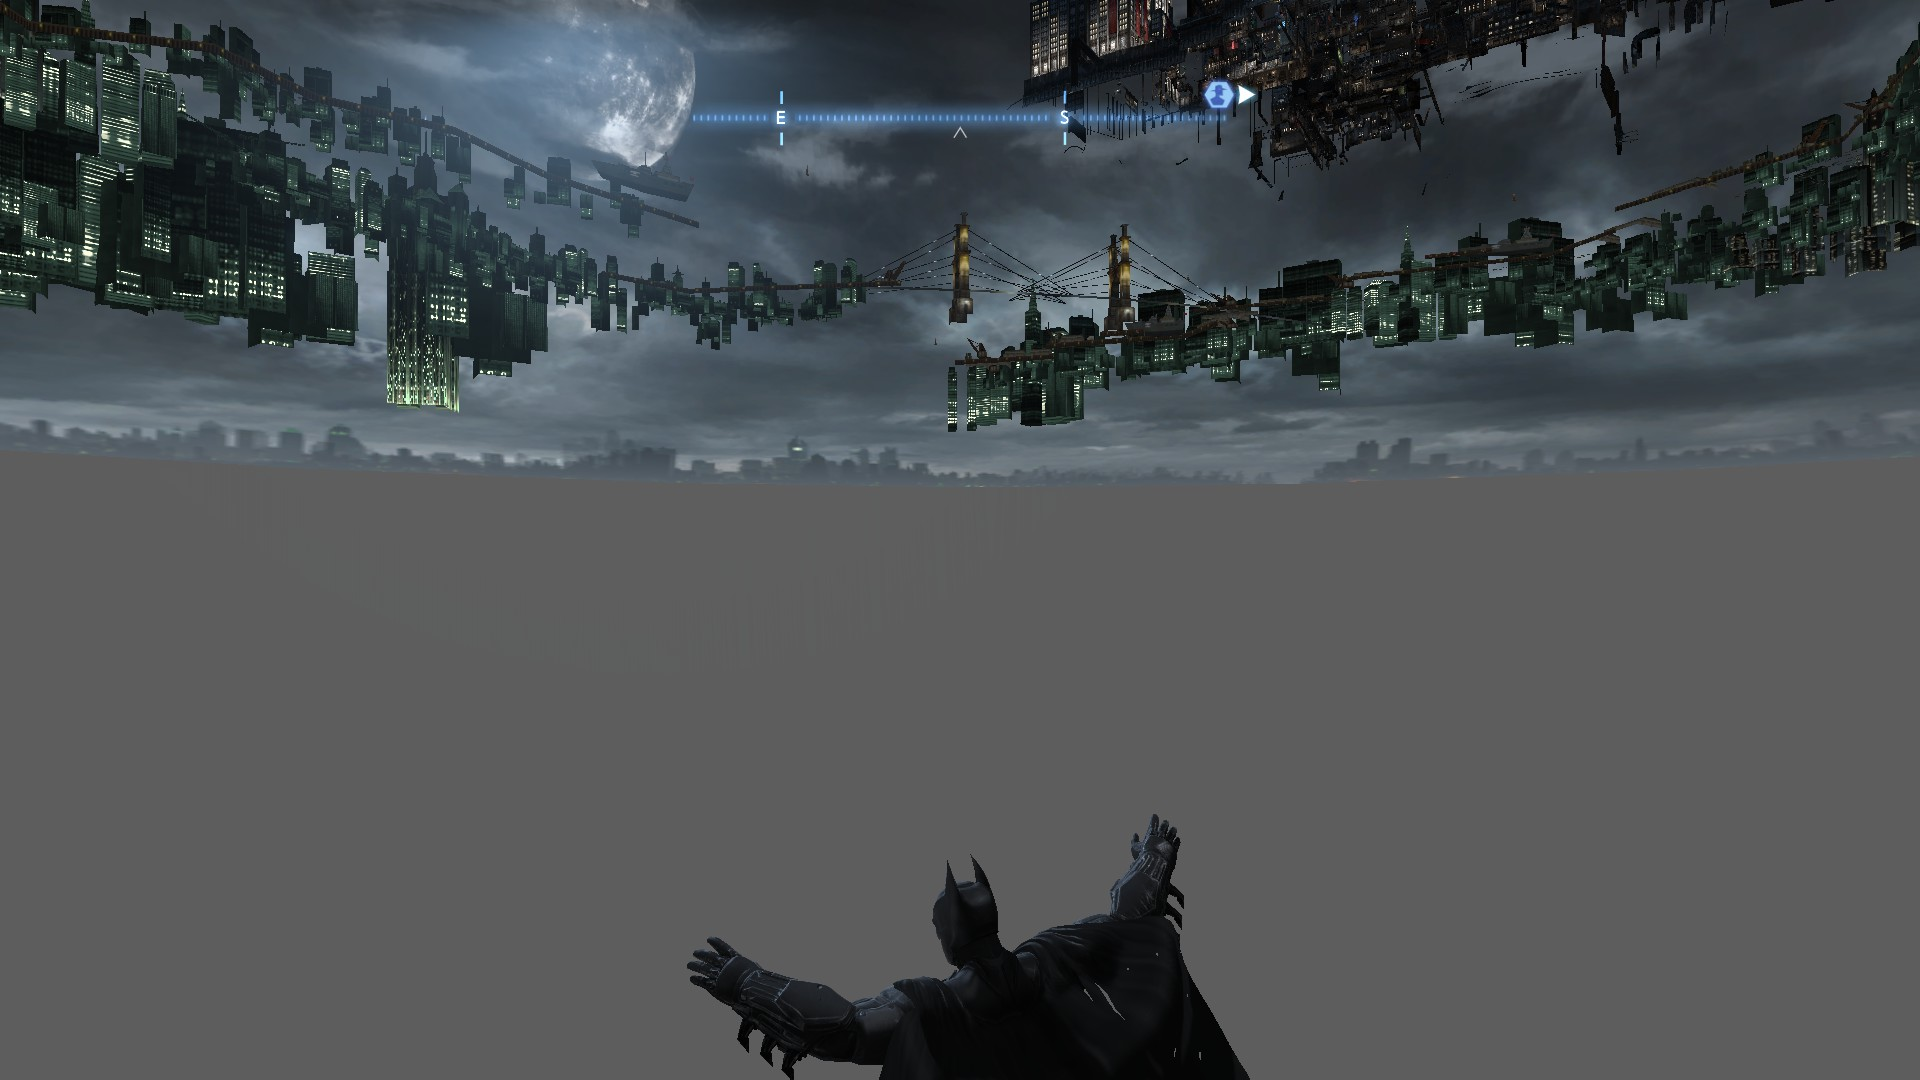
\includegraphics[scale=0.22]{batman.jpg}
\caption{Propadanje ispod modelovanog sveta.}
\label{fig:batman}
\end{figure}

\begin{figure}[h!]
	\centering
	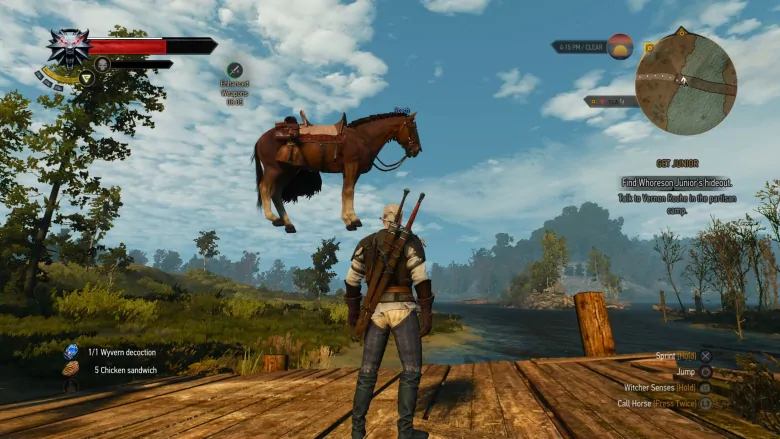
\includegraphics[scale=0.54]{horse.png}
	\caption{Levitirajući konj.}
	\label{fig:horse}
\end{figure}

Problem detekcije kolizije svih parova objekata je u najgorem slučaju kvadratne vremenske i prostorne složenosti i od toga se ne može pobeći,
ali preseka uglavnom ima mnogo manje od gornje granice. Taj najgori slučaj je na primer kada se svaka dva objekta seku.
Potreba da se algoritam izvršava u realnom vremenu je očigledna kod interaktivnih primena.
Međutim i za neinteraktivne primene, potrebno je imati što efikasniji algoritam za utvrđivanje kolizije koji bi mogao da se često pokreće.
Filmovi nisu interaktivan sadržaj i zato je učestalost osvežavanja slike od 24Hz, uz korišćenje zamućivanja pokreta (eng. {\em motion blur}),
dovoljno dobro za većinu ljudi. Standard za igre na konzolama je barem 30Hz, a na desktop računarima  barem 60Hz. 
Za primene u oblasti virtuelne realnosti potrebno je postići učestalost osvežavanja slike od barem 90Hz, jer manje frekvencije često prouzrokuju
dizorijentaciju, mučninu i druge neželjene efekte kod korisnika \cite{importance}.

Ne postoji najbolji algoritam za detekciju kolizije koji će pokriti svaki mogući slučaj. 
Neki algoritmi su dobri za uniformno raspoređene objekte u prostoru, ali pokazuju loše performanse kada su svi na jednom mestu, 
dok na druge manje utiče prostorni raspored objekata ali im efikasnost varira u zavisnosti od brzine kretanja objekata.
Takođe, isti algoritam može imati značajno bolje performanse ako su njegovi parametri dobro 
izabrani za neku hardversku arhitekturu ili okečivani raspored objekata. 
Sve pomenute činjenice inspirisale su razvoj programa koji omogućava brzo i interaktivno menjanje različitih
algoritama detekcije kolizije, postavljanje njihovih parametara kao i posmatranje performansi.

% ==============================================================================
\chapter{Pregled relevantnih pojmova}
\label{sec:karakteristike}
% ==============================================================================

U ovom poglavju biće opisani mehanizmi i fenomeni čije je poznavanje potrebno za razumevanje i konstrukciju 
efikasnog rešenja problema detekcije kolizije.
Algoritam detekcije kolizije se ne koristi kao iyolovani algoritam nego se izvršava zajedno sa renderovanjem slike,
puštanjem zvuka, mrežnom komunikacijom, rukovanjem ulaza, animacijama, simulacijom fizike, itd. 
Zato treba uzeti u obzir sve relevantne činjenice koje utiču na performanse implementacije.

\section{Faze problema detekcije kolizjie}

Celokupan zadatak detekcije kolizije se deli na dve etape: \textbf{ široku fazu } i \textbf{usku fazu}. 
U prvoj, širokoj, fazi
odbacuje se (često) većina kandidata od svih mogućih parova objekata za koje ispitujemo da li postoji presek.
Zadatak uske faze je da se za parove objekata dobijenih u širokoj fazi utvrdi da li oni zaista imaju presek.
Cilj je razviti što efikasniji algoritam prve faze (u funkciji broja objekata) za odbacivanje ovakvih parova objekata.
Iako postoje takvi slučajevi, u mnogim primenama nisu svi objekti prosta geometrijska tela poput kocki, kvadara ili lopti.
Objekti koji se razmatraju mogu biti veoma složeni, predstavljeni kao kompozicija velikog broja prostijih tela ili kao mreže sastavljene od stotina hiljada trouglova.
Mnogo je bolje razmatrati nekakvu jednostavniju reprezentaciju tih objekata.

\textbf{Granični opsezi} (eng. {\em bounding volume}) prestavljaju jedan tip jednostavnije reprezentacije.
Za granične opsege se uglavnom koristi kvadar, a pored toga se mogu koristiti sfere, kapsule i druga tela.
Ono što se najčešće radi jeste da se naprave najmanje "kutije" koje će sadržati u potpunosti te objekte.
Te "kutije" su u obliku kvadra čije su strane poravnate sa osama koordinatnog sistema i nazivaju se
\textbf{ograničavajuće kutije poravnate prema osama} (eng. {\em Axis Aligned Bounding Box}), skraćeno \textbf{ AABB }.
Umesto da se računaju preseci između velikog broja prostih objekata od kojih je telo sastavljeno, sada se posmatraju 
samo preseci među kutijama koje sadrže sve objekte.

Umesto AABB moguće je koristiti konveksne omotače tela ili \textbf{orijentisane ograničavajuće kutije} (eng. {\em Oriented Bounding Box}), skraćeno \textbf{OBB}.
\textbf{Hijerarhije graničnih opsega} (eng. {\em Bounding Volume Hierarchy}), skraćeno \textbf{BVH}, su stabla koja se grade rekurzivnom podelom 
prostora na granične opsege. Što je granični opseg bliže telima koje aproksimira to bolje, pošto to vodi do manjeg broja 
lažno pozitivnih kolizija na koje se bez razloga troši vreme u uskoj fazi. 
Reprezentacija koja koristi OBB je fleksibilnija od one koja koristi AABB pošto rotiranjem mogu uže da opišu tela. 
Ipak, zbog složenije provere preseka i zbog nepoznavanja dobrih metoda konstrukcije hijerarhije graničnih
opsega, rešenje koje koristi OBB nije nikada zaživelo u praksi \cite{obb}. 

Danas se najčešće koriste stabla izgrađena od AABB poput oktrija opisanog u \ref{subsec:octree} i njegovih modifikacija. 
Teorema o razdvajajućim osama daje inspiraciju za konstrukciju algoritma provere kolizije koristeći AABB.

\begin{teo}
	\textbf{[Teorema o razdvajajućim osama]}

	Dva konveksna objekta se ne presecaju ako postoji prava (osa) na kojoj se projekcije 
	tih objekata ne presecaju. 
\end{teo}

Nezavisno od dimenzionalnosti, razdvajajuća osa je uvek prava. Na primer, trodimenzionalan prostor
je razdvojiv ravnima, ali razdvajajuća osa je normalna na razdvajajuću ravan.

Dovoljno je pronaći samo jednu pravu tako da se projekcije tela na njoj ne presecaju.
Moguće je na primer da se uzmu normale svih strana jednog triangulisanog tela, izračunaju projekcije drugog 
tela na svaku pravu, i za neku od tih prava važi da ne postoji presek onda se razmatrana tela ne seku.
Međutim, ovakav pristup nije dovoljno dobar za potrebe detekcije kolizije u realnom vremenu. 
Zato se  ova teorema primenjuje samo za proveru preseka između AABB.

Teorema o razdvajajućim osama je takođe korisna za pronalaženje \textbf{minimalnog vektora translacije}, odnosno
vektora najmanjeg intenziteta za koji je potrebno translirati jedan objekat da bi objekti prestali da se seku.
Najčešće se simuliraju interakcije objekata koji su čvrsti i ne mogu prolaziti jedni kroz druge.
Zato je potrebno da se predstavi njihovo odbijanje promenom prvca kretanja i postarati se da ti objekati više nemaju presek.
Zbog toga, kada se ustanovi da se dva objekta presecaju potrebno je translirati ih tako da oni više nemaju presek i promeniti im vektore brzina.
Taj postupak se naziva razrešenje kolizije i opisan je u delu \ref{sec:razresenje} i u njemu ključnu ulogu igra minimalan vektor translacije.

Kada se utvrdi da postoji presek između dva AABB, to ne znači da zaista postoji presek između dva objekta
sadržana u datim AABB, čak i ako su ti objekti konveksni. Jedan takav slučaj je prikazan na slici \ref{fig:2dfalse}. 

\begin{figure}[h!]
	\begin{center}
	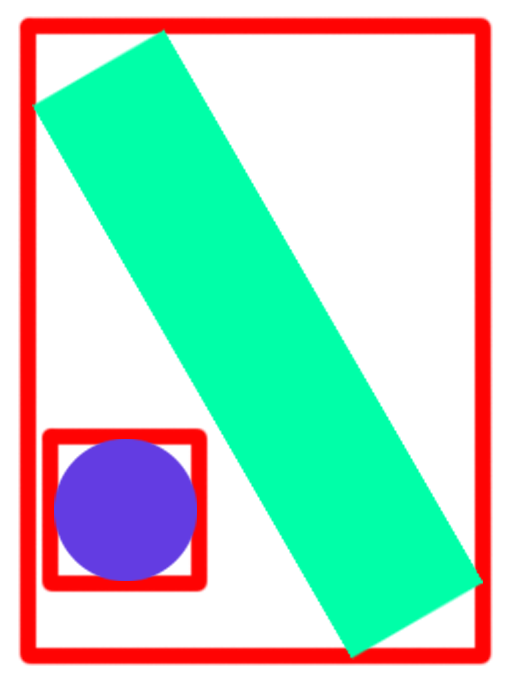
\includegraphics[scale=0.2]{2dfalseCol.png}
	\end{center}
	\caption{Krug i rotiran pravugaonik nemaju presek dok njihovi granični opsezi imaju.}
	\label{fig:2dfalse}
\end{figure}

%https://www.scss.tcd.ie/~manzkem/CS7057/cs7057-1516-07-NarrowPhase-mm.pdf
Utvrđivanje da li postoji presek objekata sadržanih u AABB koji se seku radi se u uskoj fazi.
U slučaju kada su ti objekti unutar AABB neka prosta geometrijska tela poput
lopte ili kvadra može se primeniti teorema o razdvajajućim osama da bi se videlo da li zaista postoji presek među njima. 


Međutim, nije dovoljno razmatrati samo projekcije na koordinatne ose, 
jer na primeru sa slike \ref{fig:2dfalse} vidi se da se krug i rotiran pravougaonik ne presecaju, iako se njihove projekcije 
na koordinantne ose seku. Za konveksne objekte je moguće naći neku drugu pravu koja ih razdvaja ili odrediti postojanje preseka 
na neki drugi način, ali se to ostavlja za usku fazu.

% https://en.wikipedia.org/wiki/User:Oleg_Alexandrov/Pictures
\begin{figure}[h!]
	\begin{center}
	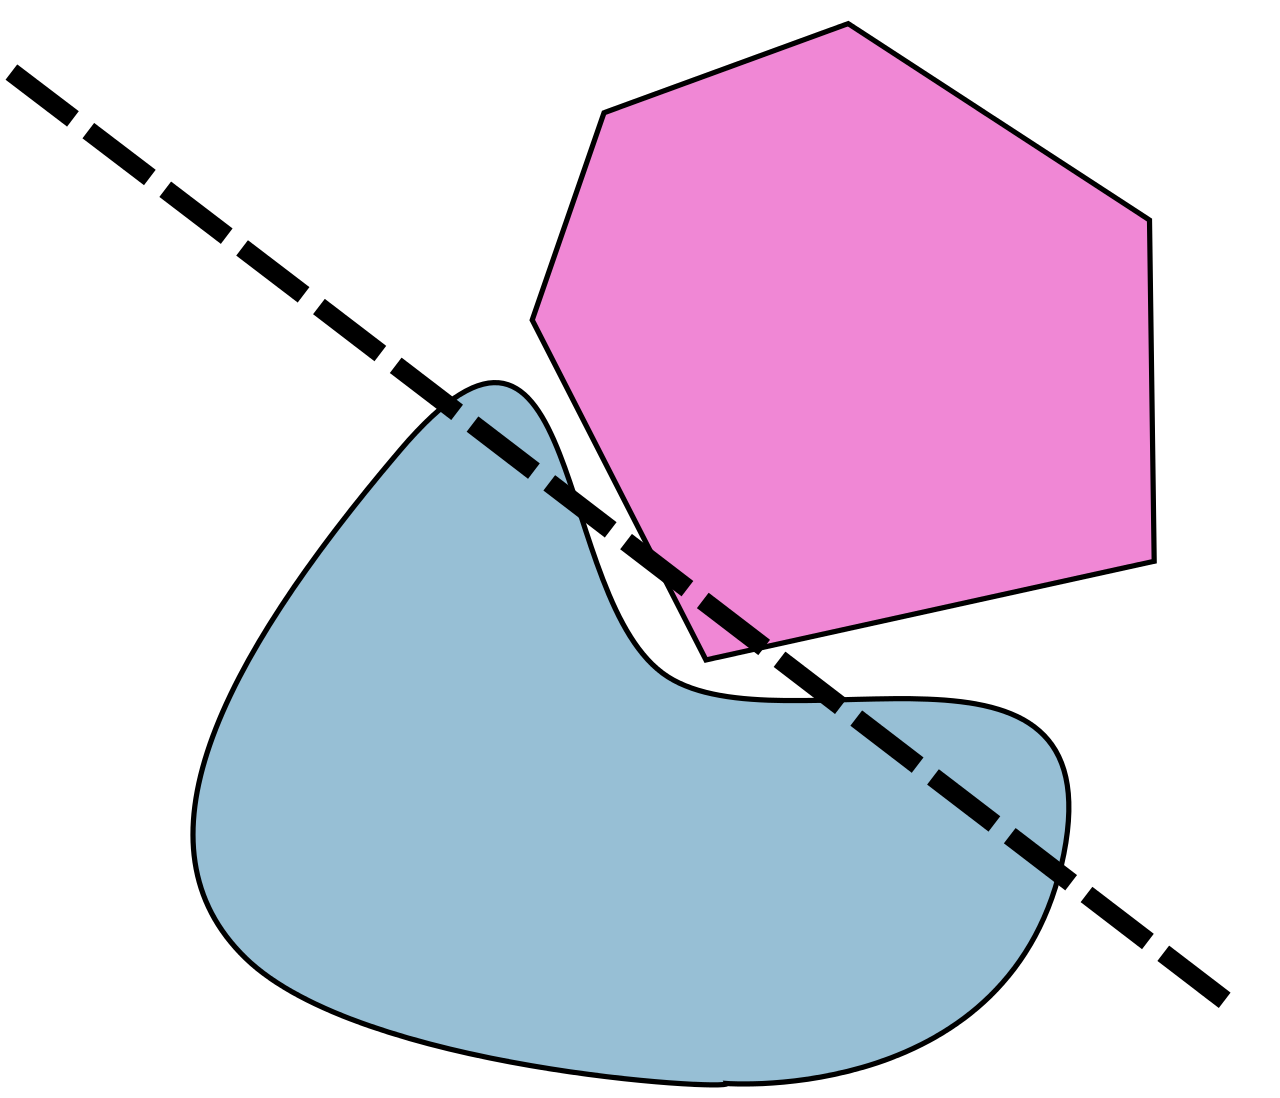
\includegraphics[scale=0.17]{theorem_counterexample.png}
	\end{center}
	\caption{Projekcija nekonveksne površi na pravu.}
	\label{fig:counter}
\end{figure}

Na slici \ref{fig:counter} prikazana su dve površi, jedna konveksna a druga nekonveksna. 
Za svaku pravu se projekcije datih površi na njoj seku, iako površi u stvari nemaju presek, što predstavlja
primer zašto teorema o razdvajajućim osama ne radi za nekonveksne objekte. 
Primer u tri dimenzije dat je na slici \ref{fig:falseCollision}, gde iako ne postoji presek dva konveksna objekta, 
posmatranjem njihovih graničnih opsega bi se zaključilo da postoji presek.

\begin{figure}[h!]
	\begin{center}
	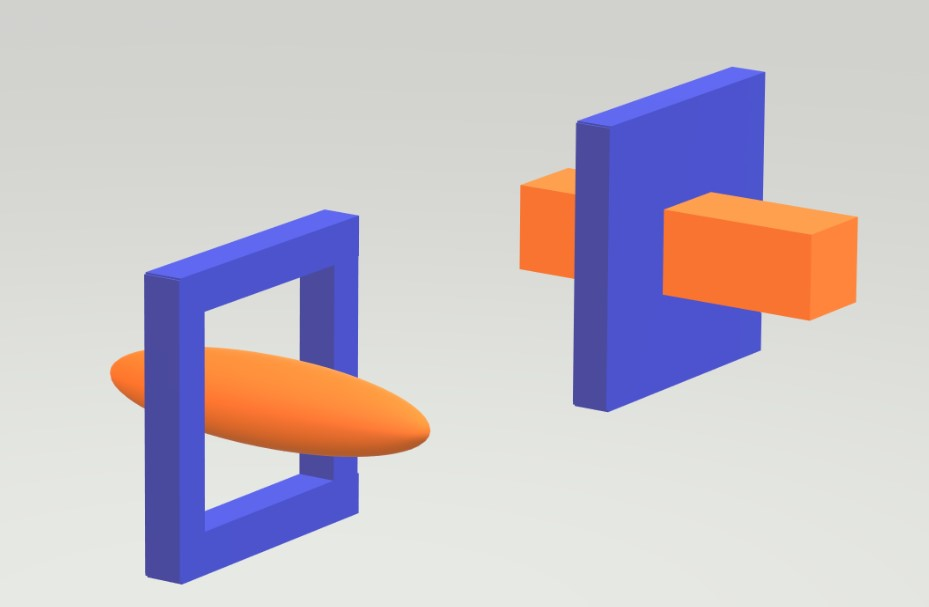
\includegraphics[scale=0.5]{falseCollision.jpg}
	\end{center}
	
	\caption{Konveksan i nekonveksan objekat u prostoru bez preseka sa leve strane i
	njihovi granični opsezi koji se presecaju sa desne strane. }
	\label{fig:falseCollision}
\end{figure}


\section{Konzistentnost vremena izvršavanja}

Prilikom razmatranja vremena izvršavanja algoritma, nekada je od interesa 
samo ukupno vreme koje je potrošeno za izvršavanje većeg broja iteracija provere da li je došlo do kolizije. 
Međutim, to nije dovoljno dobro za potrebe izvršavanja algoritma u realnom vremenu.
Ako samo jedna iteracija 
detekcije kolizije traje višestruko duže od ostalih onda dolazi do takozvanog "seckanja"
koje, ukoliko se dešava često, dovodi neupotrebljivog proizvoda.
Razmatranjem sledeće situacije se uviđa još jedan problem.

Ekrani imaju fiksnu učestalost osvežavanja koja najčešće iznosti 60Hz, mada postaju sve popularniji
% https://www.blurbusters.com/faq/120hz-monitors/
ekrani sa 120Hz, 144Hz, pa čak i 240Hz. Dakle ekran od 60Hz će svakih 16.67 milisekundi prikazati sledeću sliku. 
Ako se između dva osvežavanja ekrana uvek pripremi nova slika to je odlično. 
Još bolje da nova slika bude izračunata neposredno pre osvežavanja ekrana jer se onda 
prikazuje verodostojnija slika za taj trenutak. 
Svakako će uvek postojati neko kašnjenje od trenutka interakcije korisnika sa igrom ili simulacijom do
trenutka kada se prikaže slika, ali je cilj da to kašnjenje bude što manje. 
Kada se u jednom ciklusu osvežavanja ekrana pripremi više od jedne slike, onda se uzima ona koja je najnovija,
a prethodne se odbacuju. 
Dakle praktično je protraćeno vreme uloženo u pravljenje svih slika osim poslednje.
Kada nije izračunata nova slika za sledeći ciklus osvežavanja ekrana onda će opet biti prikazana slika
iz prošlog ciklusa. Tada se gubi na glatkoći prikazanog sadržaja i na brzini odziva programa. 

Broj slika po sekundi (eng. {\em frames per second}), skraćeno \textbf{fps}, je broj slika koje program napravi u jednoj sekundi.
Naizgled ako program ima 60fps to je savršeno za ekran od 60Hz. To ipak ne mora da bude slučaj.
U toku jedne sekunde u prvih 500 milisekundi može biti kreirano 59 slika, a u preostalih 500 milisekundi samo jedna nova slika. 
To zaista jeste 60fps, ali ono što je prikazano na ekranu nije mnogo bolje od 2fps, 
što je prektično nedopustivo. 
Dakle sa jedne strane nije dobar višak slika jer se nepotrebno troše resursi na njih iako se ne prikazuju, 
a sa druge strane manjak slika dovodi do neprijatnosti.
Zato je bitno da cela simulacija, a samim tim i detekcija kolizije ima što konzistentnije vreme izvršavanja.
Konzistentno vreme izvršavanja podrazumeva da je vreme između dve prikazane slike isto.

Na slici \ref{fig:fpsdiv2} se vidi da je kreirano 6 slika, tj. da praktično ima 6fps, iako je prikaz na ekranu 
ekvivalentan sa 3fps, što je još jedan primer nepoželjne posledice nekonzistentnosti vremena izvršavanja. 

\begin{figure}[h!]
	\begin{center}
	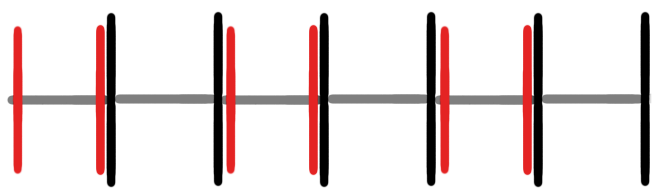
\includegraphics[scale=0.5]{fpsdiv2.png}
	\end{center}
	\caption{ Trenuci kreiranja nove slike (crvena boja) i trenuci osvežavanja ekrana (crna boja) koji su loše sinhronizovani. }
	\label{fig:fpsdiv2}
\end{figure}

\section{Vremenska koherentnost}

Često je cilj odrediti ne samo kolizije za tekuću scenu, već i kolizije u trenutku koji ubrzo sledi.
Objekti na sceni se uglavnom ne teleportuju već se postepeno kreću kako vreme teče.
Tako su pozicije objekata u bliskim trenucima slične i to se može iskoristiti za dodatno ubrzanje algoritama detekcije kolizije. 
Opšti princip je da se čuvaju svi parovi objekata koji se seku i da se u svakoj iteraciji 
izbace oni parovi objekata koji više nisu u koliziji a dodaju oni koji su od tog trenutka u koliziji.
Na taj način se značajno smanjuje vreme potrebno za izračunavanje kolizija kroz iteracije.
U slučaju da se objekti jako sporo ili uopšte ne kreću 
vremenska složenost svake iteracije algoritma biće linearna (ovo tvrđenje biće kasnije detaljnije razmatrano).


\subsection{Vremenski antialiasing}

Vremenski antialiasing ima za cilj da smanji ili ukloni efekte vremenskog aliasinga.
Vremenski aliasing nastaje kada je premali broj slika u sekundi u poređenju sa brzinom kretanja objekata na sceni.
Zbog toga objekti izgledaju kao da poskaču  umesto da odaju utisak glatkog kretanja.
Da bi se izbegao vremenski aliasing potrebno je da broj slika scene u sekundi bude bar duplo veći 
od brzine objekta koji se najbrže kreće \cite{Grant}. 
Čest primer vremenskog aliasinga je da se na snimku točkovi automobila naizgled kreću unazad.
Vremenski antialiasing se takođe koristi za smanjenje oštrih ivica koje trepere kada se pomera kamera.
Na slici \ref{fig:txaa} se vidi jasno poboljšanje kada se koristi TXAA,
tehnika koju koristi kompanija NVIDIA da bi umanjila efekat vremenskog i prostornog aliasinga.
Prostorni aliasing nastaje usled prikazivanja slike veće rezolucije na nižoj rezoluciji.
MSAA (eng. {\em multisample anti-aliasing}) je tehnika umanjenja prostornog aliasinga 
uzimanjem više uzoraka vrednosti boja u svakom pikselu.

\begin{figure}[h!]
	\begin{center}
	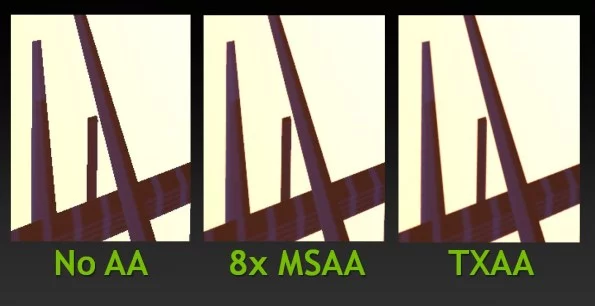
\includegraphics[scale=0.65]{txaa.png}
	\end{center}
	\caption{Upoređivanje tehnika antialiasinga.}
	\label{fig:txaa}
\end{figure}

\section{Preciznost i preseci zapremina pokretnih tela}

Koliziju je moguće utvrđivati sa različitim nivoom preciznosti. 
Pod preciznošću se misli da li su otkrivene sve kolizije koje su se desile i 
da li se objekti koji se iscrtavaju reprezentuju uprošćeno za svrhe kolizije. 
Jasno je da veća preciznost sa sobom iziskuje veće vremenske i prostorne resurse. 
Stoga se često bira nešto nepreciznija varijanta koja ima kraće vreme izvršavanja i manju potrošnju memorije.

Pošto se provera kolizije vrši u diskretnim vremenskim trenucima umesto kontinualno, može se desiti da 
je između dva uzastopna trenutka bilo kolizije, iako ni u jednom od njih nema kolizije. 
Ovaj fenomen se naziva \textbf{tuneliranje} (eng. {\em tunneling}) i ilustrovan je na slici \ref{fig:tunnel}. 

%https://github.com/Stencyl/stencylpedia/blob/master/chapter-5/ccd.md
\begin{figure}[h!]
	\begin{center}
	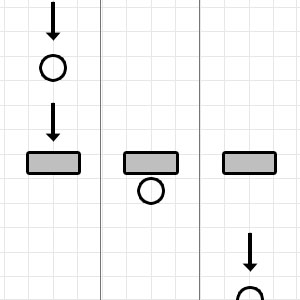
\includegraphics[scale=0.55]{tunnel.png}
	\end{center}
	\caption{Tuneliranje.}
	\label{fig:tunnel}
\end{figure}

Tuneliranje se češće javlja kod malih objekata ili kod onih koji se brzo kreću.
U oba slučaja problem je u tome što je put koji objekat pređe između dve provere kolizije velik u odnosu na veličinu objekta. 
Problem se rešava tako što se ne proverava kolizija za sâm objekat, već za celu zapreminu kroz koju je on prošao 
od prošlog trenutka provere kolizije pa do trenutnog. Na slici \ref{fig:tunnel_fix} je obojena zapremina 
koja se dodatno proverava umesto da se proverava samo objekat. 

\begin{figure}[h!]
	\begin{center}
	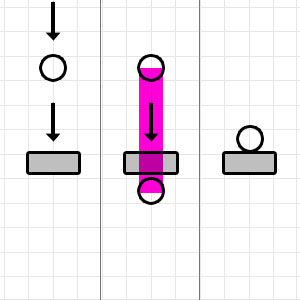
\includegraphics[scale=0.55]{tunnel_fixed.png}
	\end{center}
	\caption{Sprečavanje tuneliranja.}
	\label{fig:tunnel_fix}
\end{figure}

Pod preciznošću se može smatrati i koliko je verodostojno predstavljen model za svrhe kolizije u odnosu 
na model koji se iscrtava.
Na slici \ref{fig:hitbox} je prikazana aproksimacija kompleksnijeg modela čoveka pomoću malog broja kvadara.
Na ovaj način dobija se prostiji ali često dovoljno dobar model za detekciju kolizije koji je značajno 
jeftiniji za upotrebu u realnom vremenu. 
Nekada se ceo model čoveka aproksimira samo jednom vertikalnom kapsulom
(uglavnom za proveru kolizije modela čoveka sa statičnom geometrijom sveta). 

\begin{figure}[h!]
	\begin{center}
	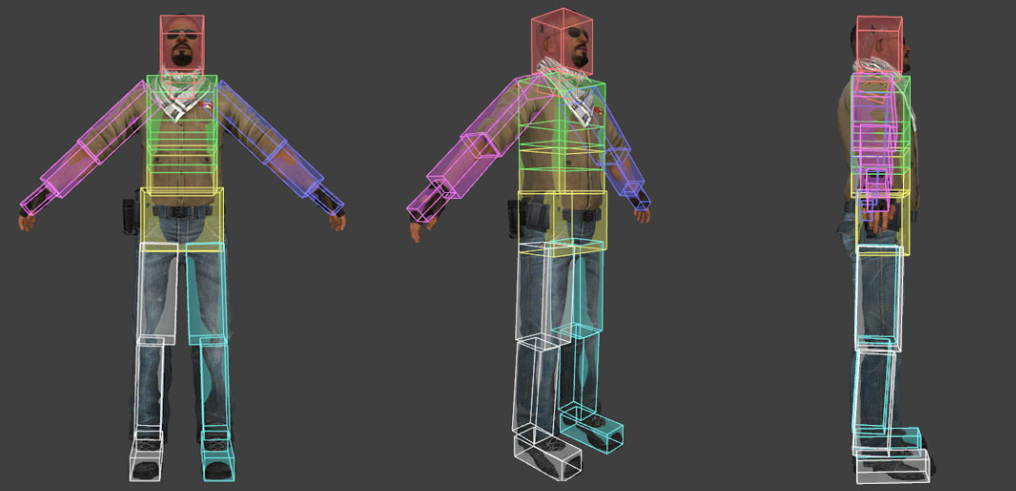
\includegraphics[scale=0.55]{hitbox.png}
	\end{center}
	\caption{Reprezentacija modela čoveka.}
	\label{fig:hitbox}
\end{figure}

\section{Izvršavanje na različitom hardveru}

S obzirom na to da se simulacija izvršava u diskretnim koracima,
bitan parametar predstavlja vremenska razlika između dva koraka.
Prevelika razlika između dva koraka je svakako nepoželjna jer je onda i prevelika razlika između dve slike scene.

Na primer, potrebno je objekat pomerati duž $x$ ose za 10 jedinica svake sekunde. Neka je interval koraka simulacije 
$p$ jednak $0.01$ sekund, onda je dovoljno da se u svakom koraku vrednost $x$ koordinate tog objekta ažurira na sledeći način:


\begin{equation}
	\label{eq:prx}
$$ x:= x + 10 * 0.01 $$
\end{equation}
% \begin{primer}
% \label{pr:x}
% $$ x:= x + 10 * 0.01 $$
% \end{primer}

Zaista, kako se pri svakom koraku $x$ uveća za 0.1, a ima tačno 100 koraka u sekundi, onda će se $x$ uvećati za 10 svake sekunde.

Poželjno je da su koraci što bliži, međutim ako bi se izabrao fiksan interval koraka $p$, onda se može desiti
da se pri određenoj konfiguraciji sistema program ne izvršava dovoljno brzo. 
Ako bi razlika između dva koraka bila $q$ gde je $q > p$, 
simulacija bi u svakom koraku napredovala za p jedinica unapred, te bi,
kako je $q > p$, simulacija izgledala kao usporeni snimak.
Nasuprot ovome, ako se ne bi stavila donja granica za vreme između dva koraka onda bi na bržim računarima
simulacija bila ubrzana. 

Jedno rešenje ovog problema se sastoji u tome da se koristi 
razlika vremena proteklog između dva uzastopna koraka, u oznaci $dt$, (eng. {\em delta time}).
Korišćenjem $dt$ je moguće izvršavanje simulacije čije vreme teče konzistentno nezavisno od broja izvršenih koraka u 
jedinici vremena. Ako je harver bolji onda će simulacija imati više koraka, odnosno više slika u sekundi, a ako je 
sporiji onda će biti manje slika u sekundi, ali vreme u simulaciji neće proticati sporije.
$dt$ bi u idealnom slučaju bilo jednako recipročnoj vrednosti broja slika u sekundi:


$$dt = \frac{1}{fps}$$
U praksi je ipak proteklo vreme između dve slike promenljivo.
Može se primetiti da dodavanjem vrednosti $dt$ promenljivoj $x$ u svakom koraku, vrednost $x$ se povećava 
za 1 svake sekunde, jer vreme svih koraka tokom jedne sekunde mora ukupno biti baš 1.
Umesto ažuriranja kao u primeru \ref{eq:prx}, sada se vrednost $x$ ažurira na sledeći način:
\begin{equation}
	\label{eq:prx}
	$$ x:= x + 10 * dt $$
\end{equation}
% \begin{primer}
% 	\label{pr:x2}
% 	$$ x:= x + 10 * dt $$
% \end{primer}

Kada se za ažuriranje svih objekata koristi ova formula, onda se simulacija može lako ubrzati $k$ puta
(množenjem vrednosti $dt$ sa $k$), odnosno usporiti $k$ puta (deljenjem vrednost $dt$ sa $k$).
Postavljanjem $dt$ na 0 svi objekti postaju statični. 
Na vrlo niskim fps igre postaju neprijatne za korišćenje, a čak mogu postati i nestabilne.
Dolazi do neželjenih efekata poput tuneliranja prikazanog na slici \ref{fig:tunnel}.
Tada se često postavlja gornja granica na $dt$, pa 
ako je vreme između dva koraka veće od te gornje granice onda će igra biti u usporenom snimku.
To je nešto što svakako nije poželjno, ali predstavlja prihvatljiviju varijantu od toga da dodje do pojave tuneliranja.

Pogon igara Unity deli sva ažuriranja na fiksna i opšta ažuriranja. 
Fiksna ažuriranja se koriste za promene sila nad objektima 
pošto se koraci u kojima se primenjuju neka pravila fizike izvode u fiksnim intervalima, 
dok se opšta ažuriranja koriste za operacije koje je potrebno izvršiti pre svakog iscrtavanja slike. 
Na primer, izmena korisničkog interfejsa igre spada pod opšta ažuriranja, a primena sile ili obrtnog momenta spada pod fiksna ažuriranja.
Unity izvršava fiksno ažuriranje i fizička izračunavanja 50 puta u sekundi, nezavisno od broja slika u sekundi \cite{unity}.
To znači da ako se igra izvršava na 25fps onda će otprilike biti dva poziva fiksnog ažuriranja na svaku iscrtanu sliku,
a ako se izvršava na 100fps tada između nekih slika neće biti nijednog fizičkog izračunavanja ni fiksnog ažuriranja.

\section{Metode za razrešavanje kolizije}
\label{sec:razresenje}

Razrešenje kolizije se sastoji od
pomeranja objekata tako da se više ne seku i postavljanja novih vektora brzina i sila koje deluju na objekte.
Nakon što algoritam detekcije kolizije odredi sve parove koji su u koliziji, 
razmatranjem svakog para se radi razrešenje kolizije svih objekata.
Postoje dva glavna načina za razrešenje kolizija \cite{Moore}.
Jedan način je da se ubaci kruta opruga između dva objekta u koliziji.
Sila opruge se primenjuje jednako u suprotnom smeru na ta dva objekta.
Smer sile je takav da što pre razdvoji objekte. Metod sa oprugama nije težak 
za implementaciju, dobar je i za čvrsta i za fleksibilna tela, ali je problem što je računski zahtevan. 
Što je kruća opruga potrebni su kraći vremenski koraci za fina numerička izračunavanja.

Drugi način je da se analitički izračunaju nova svojstva objekata u jednom koraku.
Najpre je potrebno izračunati minimalni vektor translacije. Npr. za dve sfere $s_1$ i $s_2$ to je vektor $\vec{m}$
određen centrima $c_1, c_2$ dve sfere čiji je intenzitet jednak razlici intenziteta zbira poluprečnika
$r_1, r_2$ dve sfere i intenziteta udaljenost centara, odnosno:
\begin{equation}
	\label{eq:razresenje2}
	 \vec{m} := \frac{{c_1 - c_2}} {\|{c_1 - c_2}\|} 
	(r_1 + r_2 - \| {c_1 - c_2} \| ) 
\end{equation}

Potom se jedna sfera translira za $ \frac{ \vec{m} }{ 2 }$, a druga za $ -\frac{ \vec{m} }{ 2 }$.
Sada sfere više nisu u koliziji, ali je potrebno da se promene njihovi vektori brzina nakon sudara.
Kada se koristi elastična kolizija onda se nove brzine računaju prema formulama:


\begin{equation}
	\label{eq:razresenje}
	\begin{split}
		{v}'_1= {v}_1-\frac{2 m_2}{m_1+m_2} \ \frac{\langle  {v}_1- {v}_2,\, {c}_1- {c}_2\rangle}{\| {c}_1- {c}_2\|^2} \ ( {c}_1- {c}_2) \\
		%\\
		{v}'_2= {v}_2-\frac{2 m_1}{m_1+m_2} \ \frac{\langle  {v}_2- {v}_1,\, {c}_2- {c}_1\rangle}{\| {c}_2- {c}_1\|^2} \ ( {c}_2- {c}_1) 
	\end{split}
\end{equation}


pri čemu su $m_1$ i $m_2$ redom mase sfera $s1$ i $s2$.
Analitičko izračuavanje je glavni metod koji se koristi u pogonima igara.
On je pogodniji za jake sudare, pošto je dovoljno jednom izračunati sve promene.
Ipak, za delikatnije sudare poput tela koje je polegnuto na drugo, bolje je koristiti opruge.

% ==============================================================================
\chapter{Algoritmi za detekciju kolizije}
\label{sec:algoritmi}
% ==============================================================================

Rezultat izvršavanja algoritma detekcije kolizije je skup svih parova koji su u koliziji.
U najgorem slučaju (na primer kada su svi objekti kocke na istoj poziciji) se svaki objekat
seče sa svim ostalim i tada ima $ {n\choose 2}  $ preseka, gde je $n$ broj objekata. 

Međutim, taj najgori slučaj se retko dešava u stvarnim primenama. 
Stoga, bilo bi poželjno da složenost algoritma za detekciju kolizije zavisi od broja parova objekata koji su u koliziji.
Za takve algoritme kažemo da su zavisni od izlaza, tj. njihovo vreme izvršavanja zavisi i od veličine izlaza. 
Tokom razmatranja algoritama će se podrazumevati da su svi objekti ograničavajuće kutije koje su paralelne osama,
tj. AABB. U daljem tekstu broj objekata koji se presecaju označen je sa $k$.

Pokazano je da optimalan algoritam koji pronalazi preseke $n$ AABB tela ima složenost 
$O(n \log^2 n + k)$ \cite{glavna1}. 
U praksi se obično zna u kakvim će okolnostima algoritam detekcije kolizije biti primenjen, pa 
se na osnovu toga vrši odabir postojećih ili konstruišu novi algoritmi.

\section{Osnovni algoritam}
\label{subsec:triv}

Do trivijalnog algoritma detekcije kolizije nije teško doći: za svaki element se proverava da li postoji presek sa svakim drugim elementom.
Algoritam je ispravan i njegova vremenska složenost je $\Theta (n^2) $ (gde je $n$ broj objekata), dok je prostorna složenost
$O(n^2)$, odnosno $\Theta(k)$ (gde je k broj parova objekata koji se presecaju), pošto svaki par objekata koji je u koliziji treba sačuvati.
Na složenost vremena izvršavanja ne utiču veličina objekata, njihova brzina, ni broj parova koji su u koliziji.

Pseudokod algoritma je prikazan na \ref{alg:triv}.
Glavna mana ovakvog algoritma je kvadratna vremenska složenost čak i kada nema nijedne kolizije.
Do efikasnijih algoritama može se doći particionisanjem prostora na manje potprostore, tako da
se provere kolizije vrše samo nad manjim podskupovima svih elemenata.

\begin{algorithm}
	\caption{Osnovni algoritam detekcije kolizije}
    \label{alg:triv}
	\begin{algorithmic}[1]
		\Procedure{osnovnaDetekcijaKolizije}{$objekti$}%\Comment{elements je niz svih objekata}
		\State $Parovi := \{ \}$
		\For{i:=0 to n-1}
			\For{j:=i+1 to n}

			\If{i-ti i j-ti objekti imaju presek}
				\State dodaj (i, j) u skup $Parovi$
			\EndIf		
		\EndFor
		\EndFor
		\State \textbf{return} $Parovi$
		\EndProcedure
    \end{algorithmic}
\end{algorithm}

\section{Oktri}
\label{subsec:octree}

Oktri (eng. {\em Octree}) je prostorna struktura podataka koja se koristi za rekurzivno deljenje trodimenzionog prostora na oktante.
Suštinski, oktri je stablo kod koga svaki unutrasnji čvor ima tačno osmoro dece,
što odgovara podeli prostora koji odgovara tom unutrašnjem čvoru na osam podkocki (oktanata).
U listovima se čuvaju objekti koji pripadaju oktantu koji taj list predstavlja.
%Oktri može biti tako implementiran da predstavlja i beskonačan prostor.
Na slici \ref{fig:oct} je prikazan način particionisanja trodimenizionog prostora korišćenjem oktrija.

Objekti se ubacuju u stablo počevši od korena idući rekurzivno kroz one oktante kojima objekat pripada,
sve dok se ne stigne do lista.
Pritom, postoji namenska konstanta $c$ koja sadrži vrednost najvećeg dozvoljenog broja elemenata koji list stabla može da sadrži.
Kada se prekorači taj maksimum $c$, onda list postaje unutrašnji čvor, njegov potprostor se deli 
na osam podoktanata u koje se prebacuju objekti koje je sadržao.
Potrebno je izabrati još jednu konstantu $h$ koja predstavlja maksimalnu dubinu stabla Oktrja.
Ukoliko maksimalna dubina stabla ne bi bila ograničena onda u slučaju da se ubacuje $n$ identičnih objekata (gde je $n > c$) bi se stablo 
beskonačno rekurzivno delilo pokušavajući da podeli tih $n$ objekata u različite listove 
tako da svaki ima manje ili jednako $c$ objekata u sebi. 
Pošto to nije uvek moguće konstanta $h$ zaustavlja takve podele stabla.

Parovi objekata koji su u koliziji se onda mogu pronaći na sledeći način:
kada se objekat ubaci u list, proveri se da li on ima presek sa objektima koji su već
ubačeni u taj list i svi parovi koji se seku se prijave.
Drugi način je da se prvo svi objekti smeste u oktri, 
pa da se naknadno prođe kroz sve listove i za svaka dva objekta koji pripadaju istom listu proveri da li su u koliziji.
Treba primetiti da je složenost provere kolizija kvadratna po broju elemenata u listu.
To ipak nije problem kada su elementi pretežno uniformno raspoređeni po prostoru, što je često 
i slučaj jer se uglavnom ne dopušta njihovo trajno presecanje. 

Ukoliko se razmatra tačkasti objekat, opisani postupak umetanja radi korektno,
ali se postavlja pitanje šta raditi sa većim objektima koji pripadaju više oktanata.
Jedno rešenje je da se objekat ubaci u svaki oktant kome bar delimično pripada. 
Bitan problem sa tim rešenjem je ako je u pitanju veliki objekat, onda će on pokriti mnoge oktante, njihove 
podoktante i tako rekurzivno. 
Tada veliki broj listova mora da pamti taj objekat, tj. njegovu referencu ili indeks u nekom nizu.
To nije velika smetnja kada su svi objekti sličnih veličina, ali ako 
nisu, onda i memorijska i vremenska složenost mogu eksplodirati

Drugo rešenje je da se dopusti i unutrašnjim čvorovima stabla da čuvaju objekte.
Kada neki objekat seče više od jednog oktanta nekog unutrašnjeg čvora $U$, tada se on ne ubacuje 
u podoktante čvora $U$, nego se pamti u čvoru $U$. Time se može značajno uštedeti na memoriji i vremenu izvršavanja.
Međutim, i za tako izmenjen oktri postoje nezgodne situacije kada se pogoršava vreme izvršavanja.
Ako svi objekti seku više od jednog podoktanta korenog čvora, onda svi moraju biti sačuvani u njemu. 
U tom slučaju se mora proveriti kolizija svih parova od $n$ objekata, što je ekvivalentno osnovnom kvadratnom algoritmu.

Očekivano vreme izvršavanja za izgradnju oktrija je $O(n \log n)$, gde je $n$ broj objekata.
Očekivano vreme potrebno za pronalazak svih kolizija je $O(n \log n + k)$, gde je $k$ broj objekata koji su u koliziji.

Parametri oktrija $c$ i $h$  utiču značajno na njegovu efikasnost u praksi. 
Iako broj provera u listu raste kvadratno sa $c$, to nije problem za relativno male vrednosti $c$, i često je bolje 
imati nešto veći broj elemenata u listu nego da se stablo više particioniše i duže putuje kroz njega.
Ti parametri su promenljivi u projektu i dobre vrednosti ovih parametara mogu se odrediti njihovim podešavanjem u realnom vremenu,
o čemu će biti reči kasnije.

Kada se svi objekti kreću onda se u svakom koraku simulacije  gradi novi oktri u
koga se ubacuju svi elementi i usput se odrede njihove kolizije.
Često je slučaj da je velik broj objekata statički pa je tada dovoljno jednom izgraditi oktri za njih, a za objekte koji se kreću u svakom koraku 
izvršiti detekciju kolizije njihovim ponovnim ubacivanjem u stablo. Time se smanjuje vreme izvršavanja upita 
kolizije jednog objekta koji se kreće sa $n$ statičkih sa $O(n)$ na očekivanih $O(\log n)$.

\begin{figure}[h!]
	\begin{center}
	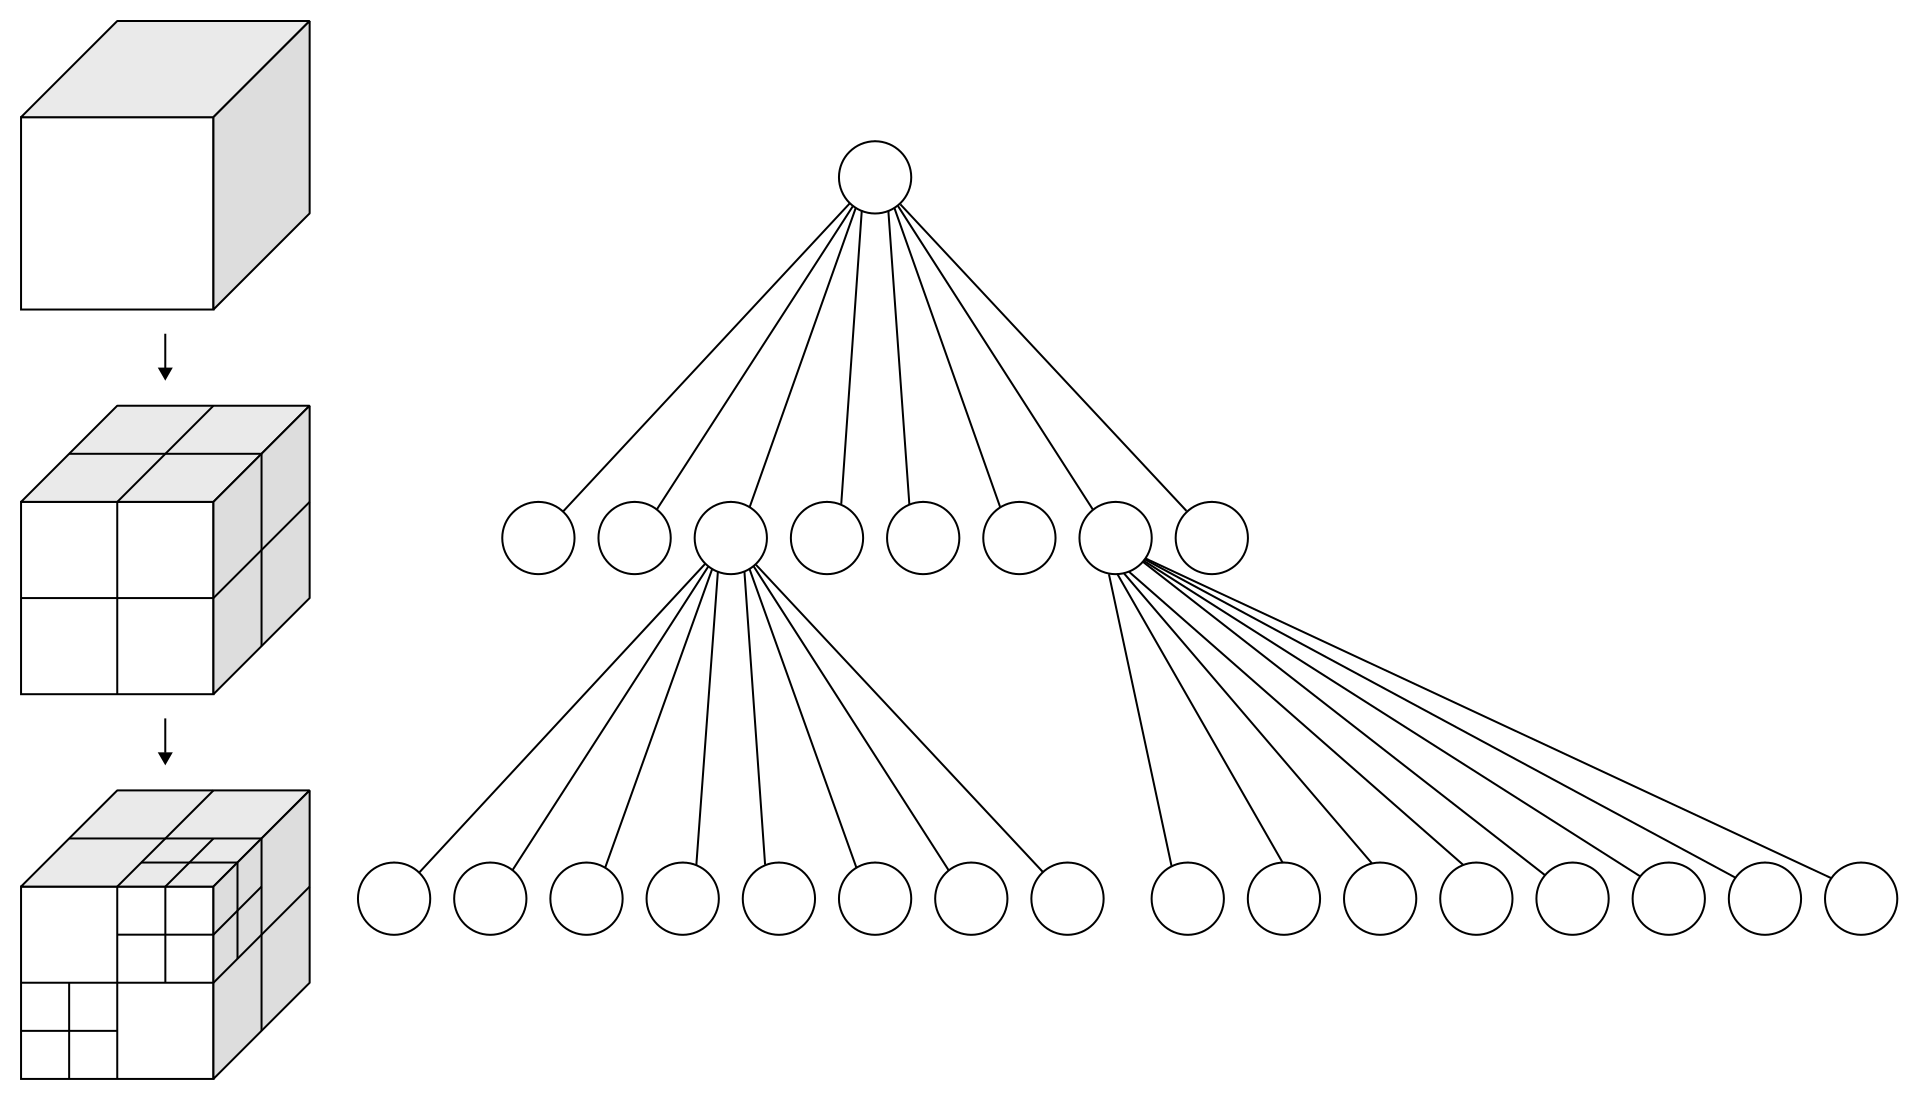
\includegraphics[scale=0.22]{octree.png}
	\end{center}
	\caption{Rekurzivno deljenje kocke na oktante.}
	\label{fig:oct}
\end{figure}

\section{Briši i odseci}
\label{subsec:sap}

Briši i odseci (eng. {\em sweep and prune}), skraćeno \textbf{SAP}, je alternativa tehnikama detekcije kolizije 
zasnovanim na prostornom particionisanju.
SAP je algoritam široke faze koji projektuje sve AABB
na bazne ose (u trodimenzionalnom slučaju to je tri skupa projekcija) pa sortira projekcije da bi odredio preseke AABB.
Ako se po sve tri ose projekcije nekog para AABB seku, onda se taj par AABB seče i u prostoru.

Ako je potrebno naći sve parove koji su u koliziji samo u jednom vremenskom trenutku onda ovaj metod ne predstavlja neko poboljšanje u odnosu na druge.
Moć briši i odseci algoritma je u tome što koristi svojstvo vremenske koherentnosti.
Objekti se ne teleportuju nasumično kroz prostor nego se postepeno kreću. 
Zbog toga je za svaku iteraciju moguće inkrementalno ažurirati parove objekata koji su u koliziji.
To se može postići na sledeći način: održavaju se tri sortirana niza, svaki od njih sadrži $2n$ elemenata, gde je $n$ broj objekata.
Svaki niz sadrži po dva elementa za projekciju svih AABB po jednoj osi: jedan element je početak 
, odnosno teme sa manjom koordinatom, a drugi je kraj projekcije, tj. teme sa većom koordinatom. 

Na slici \ref{fig:sap} je prikazana projekcija 4 objekta na jednu osu. 
Tačka $b_i$ označava početak, a $e_i$ kraj projekcije $i$-tog objekta.
U prvom momentu $e_3$ se nalazi desno od $b_4$, što posmatranjem projekcije na jednoj osi govori da su njihovi AABB možda u koliziji.
Potrebno je proveriti i ostale (ovde samo još jednu) osu sa projekcijama da bi se utvrdilo da li se stvarno seku.
Svi parovi objekata koji su u koliziji se zapamte u kolekciji parova kolizija, u ovom slučaju to je samo par $(3, 4)$.
U sledećem koraku se proverava da li je neki par koji je bio u koliziji prestao da bude, 
odnosno da li je možda neki par objekata koji prethodno nije bio u koliziji sada u koliziji.
Nakon pomeranja objekata potrebno je ažurirati projekcije objekata tako da nizovi i dalje ostanu sortirani.
Prilikom sortiranja se u stvari dodaju i uklanjaju kolizije.

Za održavanje sortiranosti se koristi sortiranje umetanjem (eng. {\em insertion sort}) 
pošto ovaj algoritam sortiranja pokazuje veoma dobre osobine za skoro sortirane nizove.
Dok se sortira niz posmatraju se elementi koji predstavljaju projekcije sleva (početak niza) nadesno i za svaki element $A$ se proverava da li treba da se elementi $B_i$ levo od $A$
pomere za jednu poziciju udesno. Postoje dva uslova koji utiču na postojanje kolizija:
\begin{itemize}  
	\item Ako je $A$ krajnja tačka projekcije a tačka $B_i$ je početna onda se par ovih objekata izbacuje iz kolekcije parova kolizije.
	Naravno prave kolizije nije moralo ni biti u slučaju da se projekcije na ostale ose ne seku, 
	pa tada izbacivanje ovog para iz kolekcije neće imati nikakvog efekta.
	\item Ako je $A$ početna tačka projekcije a tačka $B_i$ je krajnja onda se vrši provera da li se seku projekcije na ostale ose (AABB upit) i ako se seku
	onda se par odgovarajućih objekata dodaje.

\end{itemize}  


\begin{figure}[h!]
	\begin{center}
	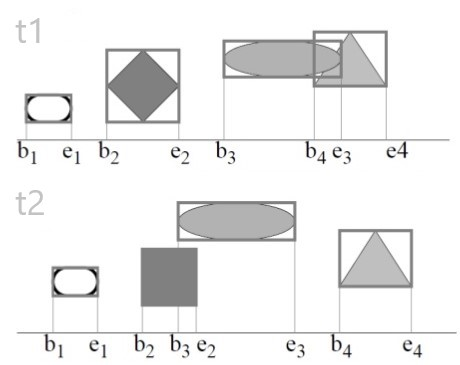
\includegraphics[scale=0.8]{sap.jpg}
	\end{center}
	\caption{Projekcije tela na jednu osu u dva koraka.}
	\label{fig:sap}
\end{figure}

Umesto da se AABB upiti vrše svaki put iznova, moguće je da se čuvaju informacije o presecima 
na svakoj osi. To zahteva $O(n^2)$ memorije ali smanjuje posao prilikom zamena \cite{sap}. 

Ovaj metod pokazuje najbolje performanse kada su objekti uniformno raspoređeni, dok mu je ponašanje lošije kada je
prisutan klaster većine objekata na nekoj osi, što vodi kvadratnoj složenosti po broju objekata \cite{glavna2}.

Prilikom evaluacije pokazuje se da najveći uticaj na performanse ima brzina kretanja objekata.
U slučaju kada se objekti brzo kreću, pomeraji objekata su veliki i potrebno je vršiti brojnije zamene njihovih pozicija u sortiranom nizu,
što vodi jakom usporavanju algoritma.
Tada svaka tačka projekcije u nizovima mora 
da se poredi sa većim brojem ostalih što dovodi do ispoljavanja kvadratne vremenske složenosti algoritma sortiranja umetanjem.
Ipak, kada se svi objekti polako kreću, onda je mali broj pomeraja u nizu, i vreme izvršavanja algoritma je praktično 
linearno, što omogućava veći broj pokretnih objekata i radi efikasnije od ostalih razmatranih algoritama u tom slučaju.

\section{Ćelije i portali}
\label{subsec:cells}

Postojanje dodatnog modela particionisanja prostora samo za detekciju kolizije nije uvek neophodno.
Postojeća hijerarhijska organizacija koja se koristi za renderovanje je nekad dovoljna.
Takva organizacija je na primer graf scene. Orgaizaciona struktura koja je vrlo pogodna
za primenu i na detekciju kolizije je metod ćelija i portala.

Ova metoda je razvijena za renderovanje sistema arhitekturalnog prolaska. 
Za njih je karakteristično okruženje koje se sastoji od velikog broja prostorija, tako da je 
većina objekata koji se nalaze u zarubljenuoj četvorostranoj piramidi pogleda (eng. {\em frustum})
nevidljivo u svakom trenutku, pošto je skoro sva vidljiva geometrija unutar trenutne sobe
u kojoj se posmatrač nalazi.
Metoda ćelija i portala deli svet u regije, odnosno ćelije, i delove koji ih spajaju, odnosno portale.
Dakle u običajenom slučaju zgrada, sobe odgovaraju ćelijama, a vrata odgovaraju portalima. 

Renderovanje scene koja je podeljena u ćelije i portale počinje prvo od one ćelije u 
kojoj se nalazi posmatrač. Nakon što je početna ćelija renderovana, poziva se rekurzivno
za susedne ćelije čiji su portali vidljivi posmatraču. Radi se presek novih portala
sa pogledom trenutnog portala čime se sužava vidljivost scene. Rekurzija se zaustavlja 
kada je presek novog portala sa trenutnim prazan, ili kada su posećene sve dostupne susedne ćelije \cite{glavnaKnjiga}.

\begin{figure}[h!]
	\begin{center}
	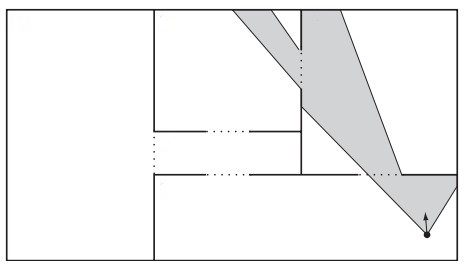
\includegraphics[scale=1]{cellsRooms.jpg}
	\end{center}
	\caption{Osenčen region predstavlja ono što posmatrač vidi. 
	Potrebno je da se renderuju samo tri od šest ćelija. }
	\label{fig:cellsRooms}
\end{figure}

Ista struktura ćelija i portala može da koristi za brzu detekciju kolizije. 
Objekti su pridruženi ćeliji gde im se nalazi centar. Kada se objekti kreću vrši 
se provera da li je objekat napustio svoju ćeliju. Ako jeste, onda se radi presek tog objekta
sa susednim ćelijama da bi se saznalo gde je otišao. 

Kada se radi detekcija kolizije između pokretnih objekata, za objekat X 
potrebno je samo proveriti objekte koji su dodeljeni istoj ćeliji kao i X, i u slučaju
da X preseca neki portal, uraditi i proveru sa objektima koji su u ćeliji sa druge strane tog portala \cite{cells}.
Traženje preseka objekata u okviru jedne ćelije zahteva kvadratan broj operacija.
Uglavnom se koristi algoritam binarnog particionisanja prostora, BSP, da bi se konstruisale
ćelije i portali.

\begin{figure}[h!]
	\begin{center}
	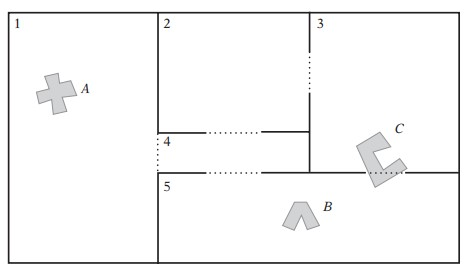
\includegraphics[scale=1]{cellsObj.jpg}
	\end{center}
	\caption{ Objekti B i C se moraju proveriti da li imaju presek, dok objekat A ne mora da se proveri ni sa jednim objektom. }
	\label{fig:cellsObj}
\end{figure}

Ova metoda se najbolje ponaša kada svaka ćelija ima isti broj objekata i kada ima dovoljno 
veći broj ćelija sa što manjim portalima.
Tada se velik broj objekata može podeliti u ćelije tako da u svakoj ćeliji ima mali broj objekata,
pa se kvadratan broj provera u okviru jedne ćelije neće naduvati.
Metoda se ne koristi u modernim igarama, ali je odlična u scenarijima za
koje je zamišljena, i daje nov način razmatranja konstrukcije rešenja za detekciju kolizije.

% ==============================================================================
\chapter{Implementacija}
\label{sec:implementacija}
% ==============================================================================

Važno pitanje na početku ovog projekta je u kom okruženju ima najviše smisla da se implementira.
Tri glavna kandidata su OpenGL, Juniti (eng. {\em Unity}) i Anril Endžin 4 (eng. {\em Unreal Engine}).

Unity i Unreal su oba pogoni igara, pa samim tim imaju sve što je neophodno da 
bi se krenuo ravoj igre ili neke druge aplikacije.
Unreal pruža mogućnost implementiranja preko shema (eng. {\em blueprints})
, preko programskog jezika C++ ili njihovom mešavinom.
Unity omogućava implementiranje pomoću programskog jezika C\# ili unityscript,
koji ima sintaksu nalik JavaSkriptu. Unityscript polako izlazi iz upotrebe, i 
sva nova dokumentacija podrazumeva korišćenje jezika C\#.
Jezik C\# u odnosu na C++ često omogućava kraće vreme implementacije nekog rešenja,
međutim postoji cena toga - nešto sporije vreme izvršavanja.
To "nešto" je uglavnom moguće ignorisati, prateći citat Donalda Knuta 
"Prevremena optimizacija je koren svog zla u programiranju".
Ipak, u slučaju programa čije performanse su od kritičnog značaja, npr. kao što je 
slučaj sa operativnim sistemima i pogonima igara, to usporenje se ne može tolerisati.
%https://en.wikipedia.org/wiki/List_of_game_engines - kako referenca za ovo
Zato su danas praktično svi pogoni 3D igara implementirani u jeziku C++.

Upravo zbog svega što pogoni igara pružaju i njihove masivnosti nisu izabrani
za osnovu implementacije ovog projekta. Oni već imaju integrisanu fiziku, detekciju 
i razrešenje kolizije. Tako bi uobičajeni kanali implementacije u njima 
bili previše indirektni za funkcionalnost koja čini srž celog sistema.
Zbog navedenih razloga je projekat napravljen korišćenjem OpenGL pomoćne 
biblioteke FriGLUT (eng. {\em FreeGLUT}) koja ima skroman skup pomoćnih funkcija
funkcija, a od ostalih je većina usmerena na grafiku i vrlo su niskog nivoa.

Ovaj projekat ne implementira algoritme detekcije kolizije u izolaziji pošto 
se oni ni neće koristiti bez ostalih komponenti kao što su iscrtavanje, 
upravljanje ulazima korisnika, razrešenje kolizije, ažuriranje pozicije i brzine objekata.

\section{FriGLUT}

FriGLUT je alternativa otvorenog koda za GLUT (eng. {\em OpenGL Utility Toolkit}). 
GLUT je prvobitno napisan da bi se podržali primeri programa u knjizi "OpenGL:
vodič za programiranje", poznatija pod nazivom "Crvena Knjiga" (eng. {\em "the Red Book" }).
GLUT se ne razvija od 1998. godine, pa je još 1999. započet FriGLUT projekat koji 
se razvija do danas. 
\cite{freeglut}

FriGLUT se stara o pravljenju prozora, obrađivanju događaja kroz glavnu petlju,
a i zajedno sa njim su dostupne i standardne funkcije OpenGL-a koje se koriste
za iscrtavanje poput glTranslatef, glScalef, glLightf, glMaterialfv, glViewPort, itd.
Za odgovore na događaje pritiskanja tastera, puštanja tastera i pomeraja miša
FriGLUT propisuje korišćenje funkcija povratnog poziva  (eng. {\em callbacks }) koje je potrebno implementirati.
FriGLUT se ne stara o tome da li je u nekom trenutku neko dugme pritisnuto, 
koliki je pomeraj miša, niti ga automatski repozicionira, ali barem pruža 
funkcije koje su neophodne da bi se to ostvarilo.

\section{Arhitektura}

Glavne komponente programa su:
\begin{itemize}
	\item Komponenta za iscrtavanje
	\item Komponenta za rukovanje ulazima korisnika
	\item Centralna komponenta - poziva sve ostale komponente i stara se o vremenskim koracima
	\item Kontroler komponenta za upravljanje svim parametrima algoritama
	\item Komponenta za merenje performansi
	\item Komponenta za ažuriranje brzine i pozicije objekata
\end{itemize}

\begin{figure}[h!]
	\centerfloat
% https://online.visual-paradigm.com/w/jllvezfo/diagrams.jsp#diagramlist:open&mode=Local
	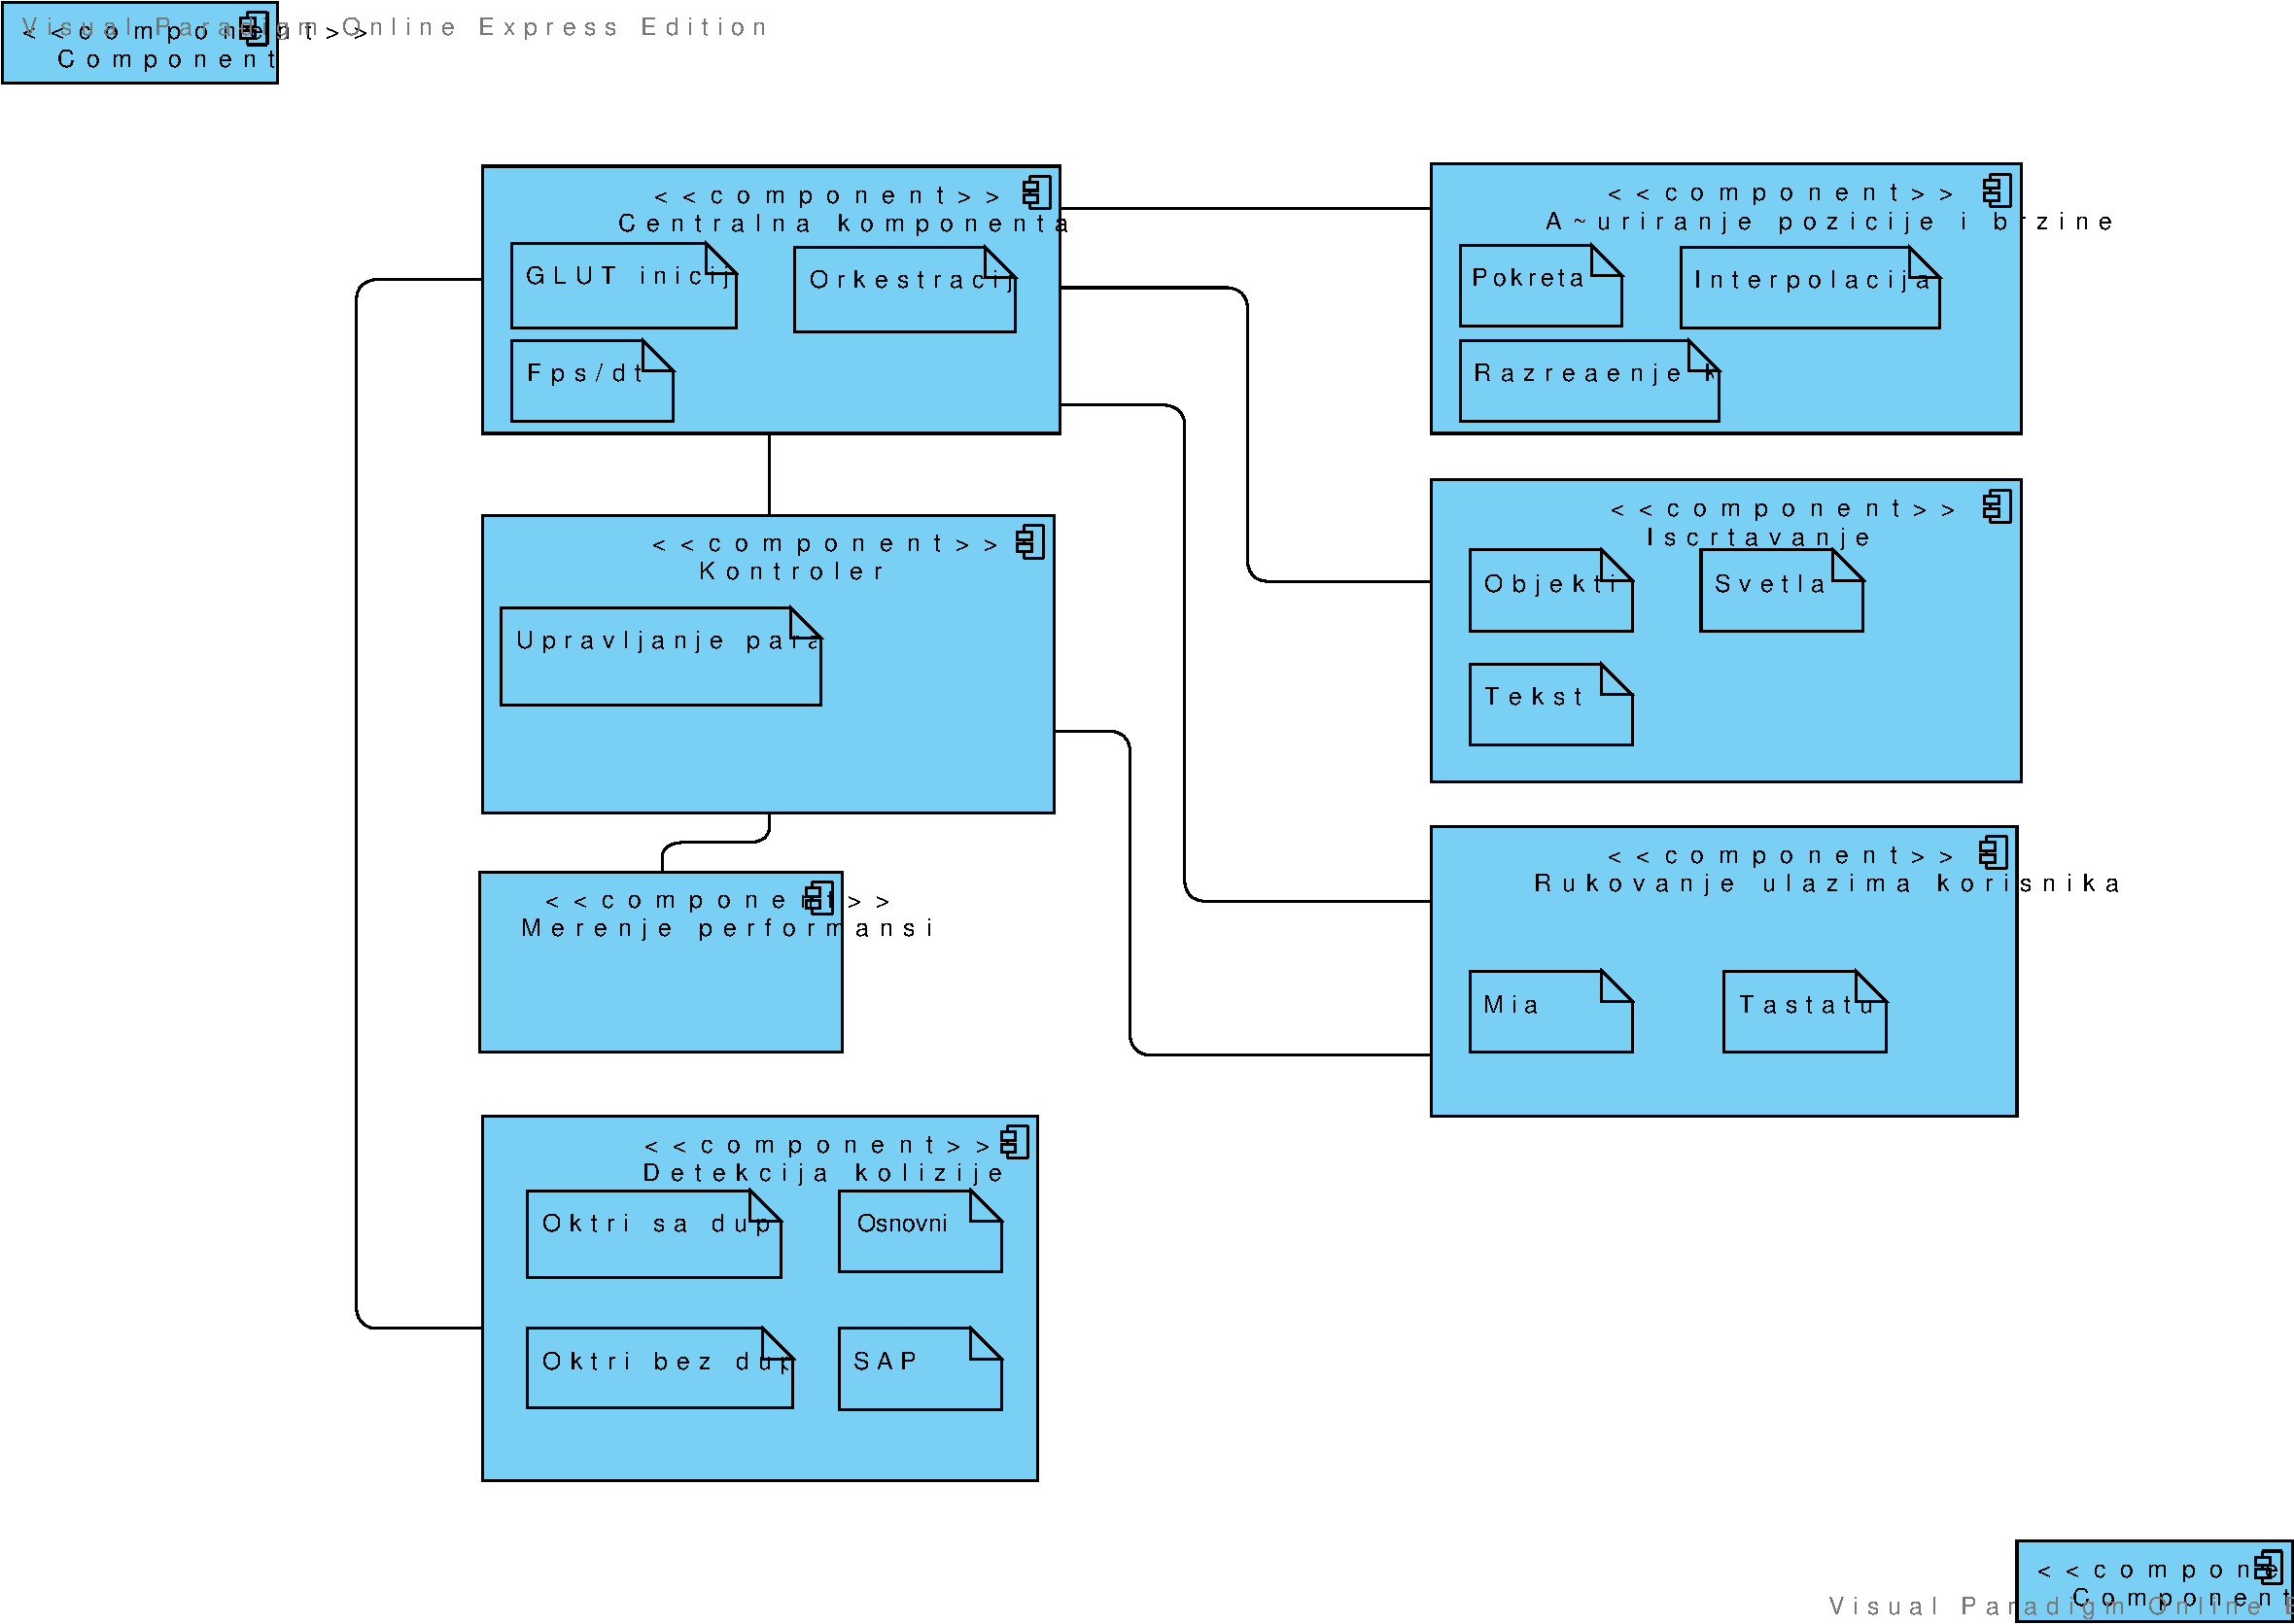
\includegraphics[trim=150 50 100 50,clip,scale=0.6]{architecture.pdf}
	\caption{Arhitektura.}
	\label{fig:archi}
\end{figure}

Na slici \ref{fig:archi} je prikazana arhitektura programa sa navedenim komponentama.

\subsection{Kontroler komponenta}

Parametri koji se menjaju kroz kontroler komponentu su: 
\begin{itemize}  
	\item Broj objekata koji su podložni koliziji. 
	Ovo je parametar koji svakako najviše utiče na ponašanje algoritama.
	\item Veličina objekata. 
	Na prvi pogled liči da ne bi mnogo uticalo na perofmanse, međutim veliki objekti u malom prostoru mogu katastrofalno usporiti izvršavanje.
	\item Brzina kretanja objekata.
	Ovaj faktor ne utiče na mnoge algoritme, ali je u slučaju SAP algoritma najbitniji. Može promeniti odlično ponašanje SAP algoritma u slučaju sporog kretanja 
	objekata i učiniti ga praktično algoritmom kvadratne složenosti u najgorem slučaju.
	\item Veličina kontejnera u kome se nalaze i kreću svi objekti.
	Daje još jednu perspektivu kako veličina objekata i odnos te veličine sa celim prostorom, ovde kontejnerom, utiču na performanse.
	\item Maksimalan broj elemenata u listu oktrija.
	Promena maksimalnog broja elemenata u listu pre nego što se on podeli na podoktante utiče "samo" na konstantan faktor vremenske složenosti.
	To uopšte nije zanemarljivo u datom kontekstu i povoljnosti koje daje povoljno izabran parametar su vrlo vidne.
	\item Maksimalna dubina oktrija. Što veća dubina je uglavnom povoljnija, mada treba biti oprezan ako se može desiti 
	da se velik broj objekata preklapa unutar jednog oktanta, jer se tada samo gubi vreme i troši dodatna memorija. 
	Pokušavaju se razdvojiti objekti rekurzivnom podelom potprostora, ali pošto se oni presecaju taj put je beznatežan.
	\item Da li raditi razrešenje kolizije. 
	Razrešenje kolizije je odvojen problem od detekcije kolizije, a pošto se uglavnom koriste oba, onda je dobro videti 
	kako razrešenje kolizije deluje na performanse detekcije kolizije. Praktično uvek deluje povoljno, pošto onemogućava da se mnogo 
	objekata međusobno preseca, pa time smanjuje verovatnoću da se stvori veliki klaster objekata koji bi usporio izvršavanje.
	\item Da li je iscrtavanje uključeno ili isključeno. 
	S obzirom da je projekat više procesorski nego grafički zahtevan, iscrtavanje uglavnom ne oslabljuje performanse više od 2 do 3 posto.
	Svakako, kada je na sceni više od 30 000 objekata počinje značajno da ima uticaj, pa je za te slučajeve dodata opcija kako bi merenja bila nepristrasna.
	\item Koji algoritam detekcije kolizije se koristi. Podržani su: osnovan (trivijalan) algoritam, oktri sa duplikatima,
	oktri bez duplikata i SAP algoritam. Takođe je moguće isključiti detekciju kolizije u celosti da bi se dobila referntna vrednost vremena izvršavanja.

\end{itemize}  

Kontroler komponenta takođe pruža mogućnost menjanja pravca kretanja objekata. 
Tada svi objekti bivaju usmereni prema trenutnoj poziciji posmatrača. 
Potrebna je takva funkcionalnost pošto ona povećava koncentraciju objekata, 
pogotovo nakon što se odbiju o ivicu kontejnera. Tada će se većina objekata 
naći oko centra kontejnera, što dovodi do eksplozije vremena izvršavanja, pogotovo u slučaju oktrija sa duplikatima.

\subsection{Komponenta za iscrtavanje}

Sve što se želi prikazati mora se iskazati preko GL funkcija. 
Boje objekata zavise od osvetljenja i materijala ili teksture koja mu je dodeljena.

Ljudska percepcija boje objekta je zapravo spektar elektromagnetnog zračenja koji se odbija o taj objekat i pada na retinu oka.
U pravom svetu se zraci svetlosti odbijaju od više objekata pre nego što stignu do oka. 
Simulacija takvog ponašanja se naziva praćenje svetlosti (eng. {\em raytracing}).  
Praćenje svetlosti je računarski zahtevno, pa do skoro nije bilo moguće izvršavati ga u realnom vremenu, već samo na farmi servera koji renderuju neku scenu.
2018. godine je firma NVIDIA pustila u prodaju novu seriju grafičkih karti koje hardverski implementiraju praćenje svetlosti. 
U trenutku pisanja se ova tehnologija koristi kao hibrid, odnosno ne kao zamena nego dopuna postojećih metoda.

Uobičajeno je da se materijali objekata opisuju pomoću Fongovog modela senčenja. 
Fongov model je empirijski model osvetljenja. Razvio ga je Bui Tuong Fong i objavio ga u svojoj doktorskoj tezi 1975. godine.
Opisuje boju površi kao kombinaciju difuzne refleksije, tj. odbijanja svetlosti sa grubih površi, 
spekularne refleksije, tj. refleksija sa sjajnih površi, i ambijantne refleksije, koja predstavlja manju količinu svetlosti 
koja je raspršena kroz celu scenu.
\cite{Phong} OpenGL nudi Fongov model pa se on koristi za opisivanje materijala svih objekata.
Todo slika možda.
Uključeno je jedno globalno svetlo, a moguće je da posmatrač postavi jos najviše osam svetala na 
proizvoljne statične blokove na mapi. 
Slabljenje svetlosti se izražava preko tri faktora: konstantnog, linearnog i kvadratnog.
Konstantan faktor jednako oslabljuje svetlost svuda, dok linearni i kvadratni faktori oslabljuju svetlost
linearno, odnosno kvadratno, sa rastojanjem od izvora svetlosti.

Komponenta se brine i o iscrtavanju teksta, što zahteva nešto više gl poziva nego što bi se očekivalo.

Postavljanje kamere zavisi od pozicije posmatrača i njegovog usmerenja pogleda levo-desno i gore-dole.
Kamera se usmerava od pozicije posmatrača ka pravcu u kome gleda.
Vektor pravca gledanja se dobija prema formuli:

\begin{equation}
\label{eq:camera}
\begin{split}
x = cos(hrot) \cdot cos(vrot) \\
y = sin(vrot) \\
z = cos(hrot) \cdot  cos(vrot)	
\end{split}
\end{equation}


Gde je $vrot$ ugao između $xz$ ravni i pravca gledanja, dok je $hrot$ ugao rotacije oko $y$ ose.
Napomena da je u OpenGL-u $y$ osa vertikalna, $x$ horizontalna, a $z$ predstavlja dubinu.

\subsection{Centralna komponenta}

Centralna komponenta inicijalizuje GLUT funkcije povratnog poziva, postavlja GL parametre, i pokreće sistem.
Definiše tajmer koji će periodično pozivati ažuriranje sistema i zakazati njegovo ponovno iscrtavanje. 
Stara se o računanju vremena dva uzastopna koraka izvršavanja, redosledu pozivanja ažuriranja stanja,
detekcije kolizije, razrešavanja kolizije i iscrtavanja.

\subsection{Komponenta za ažuriranje brzine i pozicije objekata}
% ona radi i razresavanje kolizije

Svaki objekat sadrži trojku brojeva u pokretnom zarezu koja označava njegovu poziciju za svaku koordinatu prostora.
Za održavanje pravca je potrebna još jedna trojka koja predstavlja vektor brzine kretanja.
Ako se pritom želi da objekat postepeno ubrzava kada se primeni sila na njega, ili da postepeno usporava 
kada prestane delovanje sile, onda se mora čuvati još jedna trojka brojeva, koja predstavlja ciljnu brzinu.
Postepeno ubrzavanje se koristi prilikom upravljanja posmatrača. 
Kada se pritisne dugme na tastaturi za pomeranje posmatrača, očekivano ponašanje je da neće istog trenutka 
početi da se kreće maksimalnom brzinom, već postepeno da ubrzava.
Isto, kada se pusti dugme, "sila" koja je delovala na posmatrača je nestala, ali je on imao momentum pa će
nastaviti malo napred.

Potrebno je posvetiti pažnju kako se posmatrač kreće na komandu da ide napred-nazad ili levo-desno.
Prva ideja bi bila da se za kretanje levo-desno poveća ili smanji vrednost pozicije $x$ koordinate posmatrača,
ili da se menja $z$ koordinata posmatrača kada treba da se kreće napred-nazad.
To ipak nije dobro rešenje pošto kada neko želi da se pomeri ne razmišlja preko strana sveta na koju će stranu, 
već relativno u odnosu na trenutnu njegovo usmerenje. Usmerenje je dato formulom \ref{eq:camera}.
Neka je dat trodimenzioni vektor $v$ koji predstavlja usmerenje pogleda, tada je vektor 
kretanja unapred jednak: 
$$ v_{napred} = \frac{(v_1, 0, v_2)^T}{\|(v_1, 0, v_2)^T\|} $$
Pritom se normira vektor kako se ne bi sporije kretalo u slučaju gledanja gore ili dole, 
pošto su tada $v_1$ i $v_2$ mali.
Slično, vektor kretanja u stranu se računa kao:
$$ v_{bok} = \frac{(-v_2, 0, v_1)^T}{\|(-v_2, 0, v_1)^T\|} $$

Sada su zamenjene vrednosti prvog i trećeg elementa vektora zato što kada se gleda pravo u smeru $x$ ose, 
onda je bočno kretanje duž $z$ ose. Razlog za promenu znaka $v_2$ je jednostavno zbog orijentacije $z$ ose u odnosu na $xz$ ravan.
Koordinatni sistem koji se koristi je prikazan na slici \ref{fig:coord}.

\begin{figure}[h!]
	\centerfloat
	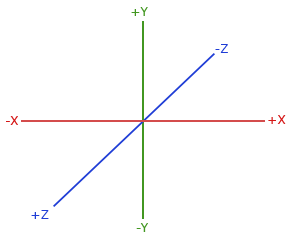
\includegraphics[scale=1]{coord.png}
	\caption{OpenGL koordinatni sistem.}
	\label{fig:coord}
\end{figure}

Kontejner koji sadrži objekte koji se sudaraju se stara o njihovom pravilnom odbijanju o ivice ograničavajućeg prostora.
Svakako, potrebno je reflektovati dimenziju vektor brzine koja odgovara osi duž koje se objekat sudara sa ivicom kontejnera.
Objekti će nekada delom zaći van kontejnera, pa se tada oni pomere u unutrašnjost tako da jedna njihova strana bude uz stranu kontejnera.

Kada se na primer na kuglu koja stoji uz zid primeni sila koja nije normalna na stranu zida, onda kugla neće ostati nepokretna,
već se kretati paralelno uz stranu zida. Isti princip je obezbeđen za kretanje posmatrača uz zid jer je 
takvo ponašanje standardno za sve video igre.

Detekcija kolizije kao rezultat daje parove svih objekata u koliziji. Na te parove se primenjuje 
razrešenje kolizije prema formulama \ref{eq:razresenje} i \ref{eq:razresenje2}.

\subsection{Komponenta za merenje performansi}
\label{sec:perf}

Služi za prikupljanje podataka kako bi se uradila evaluacija data u \ref{sec:evaluacija}.
Jedna instanca merenja predstavlja jedan korak izvršavanja i sastoji se od 
vremena izvršavanja koraka, veličine objekta, broja objekta, dodatnih podataka u zavisnosti od toga 
koji algoritam detekcije kolizije se koristi. Ne zapisuje se direktno u izlaznu datoteku, pošto bi 
to usporavalo izvršavanje, već se čuva u vektoru, pa se napravi datoteka u koju se zapišu rezultati 
tek kad je gotovo merenje.

\subsection{Komponenta za rukovanje ulazima korisnika}

Definiše funkcije povratnog poziva koje će FreeGLUT pozivati.
Potrebne su funkcije za akciju pritiska dugmeta tastature, puštanje dugmeta, kao i 
radnja koja se vrši dok je dugme pritisnuto. Za poslednju stavku se mora ručno implementirati 
za svako dugme pamćenje stanja pritisnutosti. Ako se želi akcija na pritisak specijalnih dugmeta  
poput F1, F5, strelice i slično, onda se zahteva definisanje odvojenih funkcija za njih.

Što se tiče reakcija na pritisnuto dugme, prva ideja je da se direktno pozove ta akcija. 
To je u redu ako je ta akcija na primer izlazak iz programa, promena izabranog algoritma, ili neka druga jedinična akcija.
Ako je pak slučaj akcije poput kretanja napred, onda bi takvo ponašanje imalo neprijatan efekat. 
Osljanjalo bi se na učestale ponovljene signale da je dugme pritisnuto, koji u praksi uopšte nisu periodični.
Tada bi kretanje "seckalo", i njegova brzina bi zavisila od mogućnosti glavne petlje događaja da signal pritiska dugmeta često i ravnomerno poziva.
Ili obrnuto, mogla bi se desiti dva uzastopna signala pritiska dugmeta za napred između dva iscrtavanja scene. 
Da li bi tada trebalo da se napravi duplo veći pomeraj? Odgovor je ne, ali bi to bio efekat ovakve implementacije.

Ispravno rešenje je da se zapamti da je dugme pritisnuto, a onda da se reakcija na to desi tek zajedno sa ostalim ažuriranjima 
stanja i pozicija, što se dešava periodičnim pozivima komponente koja je za to zadužena. Tako je reakcija nezavisna od učestalosti 
slanja ponovnih signala da je dugme pritisnuto, štaviše, oni su sada nepotrebni. 

Što se tiče miša, postoje tri funkcije koje je potrebno implementirati. Prva je za akcije pritiska 
dugmeta miša, druga je za pomeraj miša, i treća je za pomeraj miša dok je neko dugme na njemu pritisnuto.
Potrebno je pratiti veličinu svakog pomeraja miša i na osnovu toga izračunati novu horizontalnu i vertikalnu rotaciju 
kamere, odnosno posmatračevog usmerenja. Kako kursor miša ne bi napustio prozor programa, potrebno je da se on nakon svakog pomeraja 
vrati u centar prozora. Kursor miša je takođe sakriven, a dodata je opcija da se prikaže i da dobije nazad slobodu da napusti prozor.

\subsection{Komponenta za detekciju kolizije}

Za projekat najznačajnija funkcionalnost dolazi od ove komponente. 
Algoritmi su implementirani u odvojenim klasama, ali imaju isti interfejs.
Svaka klasa implementira metodu kojoj se prosleđuje vektor objekata za koje treba proveriti da li su u koliziji
i vraća sve parove objekata koji jesu u koliziji. Takođe svaka implementira metod koji daje relevantne podatke 
o stanju algoritma specifičnom za njega. Npr. broj elemenata u unutrašnjim čvorovima oktrija ili broj 
zamena u SAP algoritmu. Oni se koriste za merenje i za ispisivanje trenutnih informacija prilikom testiranja.

% ==============================================================================
\chapter{Evaluacija}
\label{sec:evaluacija}
% ==============================================================================

U ovom poglavlju će biti izloženi rezultati merenja vremena izvršavanja koraka simulacije.
Da bi se dobile vrednost $dt$ koje predstavljaju proteklo vreme između dva uzastopna ažuriranja scene
koristi se komponenta \ref{sec:perf}, a za dobijanje preciznog trenutnog vremena se koristi funkcija iz GLUT biblioteke.
U daljem tekstu se pod "relativan $dt$" podrazumeva:
$$ \frac{ dt }{16.667} $$

Razlog za deljenjebrojem 16.667 je taj što je poželjan minimalan broj iscrtavanja u sekundi 60, 
što je $1/60$ u terminima proteklog vremena $dt$.

Sva merenja su izvršena na računaru sa sledećom konfiguracijom:
\begin{itemize}  
	\item Procesor - Intel Core i5-6600K 
	\item Grafička - NVIDIA GeForce GTX 1060 WINDFORCE OC 6G
	\item RAM - Kingston HyperX FURY 8GB 2133MHz DDR4 
	\item Matična - ASUS Z170-A
\end{itemize}  
Pritom se pazi da nisu pokrenuti drugi programi koji bi uticali na rezultate.
Procesorski takt je postavljen na 4.4 GHz.

Za preprocesiranje i prikaz podataka korišćen je programski jezik \textbf{Python},
biblioteka \textbf{pandas} za manipulisanje podacima i biblioteka \textbf{matplotlib}
za pravljenje grafika.

\section{Opšte}

Za početak, potrebno je ustanoviti koliki uticaj ima postupak iscrtavanja na vreme izvršavanja.
U slučaju da iscrtavanje troši veći ili približan deo vremena u odnosu na detekciju kolizije, onda 
bi bilo nepravilno meriti ih zajedno. Zato je obezbežen način da se isključi iscrtavanje ako bi se to dešavalo.


Na slici \ref{fig:drawVsNoDraw} i sledećim graficima su date referentne vrednosti:
\begin{itemize}  
	\item Prava koja predstavlja linearnu zavisnost $y$ od $x$ prikazana isprekidanom zelenom bojom.
	Prava je sa koeficijentom pravca jednakim $y_0/x_0$.
	\item Ciljna vrednost od 60 slika po sekundi prikazana žutom bojom.
	60 slika po sekundi je traženi minimum za računare.
	\item Ciljna vrednost od 30 slika po sekundi prikazana crvenom bojom.
	30 slika po sekundi je traženi minimum za igre na konzolama.
\end{itemize}  

\begin{figure}[h!]
	\centerfloat
	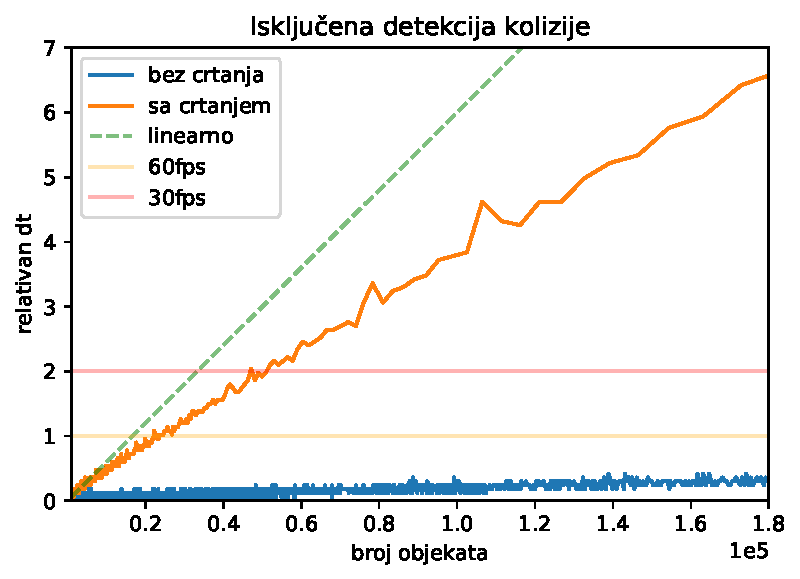
\includegraphics[
		trim= 0 0 0 19, clip,
		scale=1]{idleDrawVsNoDraw.pdf}
	\caption{Relativan dt u zavisnosti od broja objekata - isključena detekcija kolizije.}
	\label{fig:drawVsNoDraw}
\end{figure}

Na slici \ref{fig:drawVsNoDraw} prikazan je grafik zavisnosti relativnog dt u odnosu na broj objekata.
Detekcija kolizije je isključena, tako da na vreme utiče samo kretanje objekata i iscrtavanje.
Kada je iscrtavanje uključeno onda vreme izvršavanja raste linearno (sa koeficijentom manjim od 1).
Na oko 24 000 objekata relativan dt prelazi 1, a na 50 000 objekata dt prelazi 2. 
Sa druge strane, kada je crtanje isključeno vreme izvršavanja je mnogo manje. Svakako raste linearno 
sa brojem objekata, ali sa konstantom koja je preko red veličine manja od iscrtavanja. 
Čak i kada ima preko 180 000 objekata program se izvršava sa malim relativnim dt, 
što znači da je to vreme zanemarljivo u odnosu na vreme potrebno za detekciju kolizije.

Na slici \ref{fig:basic} prikazana je zavisnost relativnog dt od broja objekata kada se koristi 
trivijalan algoritam kolizije. Na grafiku se naravno vidi nagli rast, što je i očekivano pošto 
je algoritam kvadratne vremenske složenosti. Čak pre 2000 objekata relativan dt postaje veći od 1, 
a na 2500 veći od 2. Takvo rešenje je neupotrebljivo za veći broj objekata. Jedina "prednost" je što 
je složenost vremena izvršavanja ista koliko god da se brzo objekti kreću, koje god da su veličine i koliko god 
da ih se preseca.

\begin{figure}[h!]
	\centerfloat
	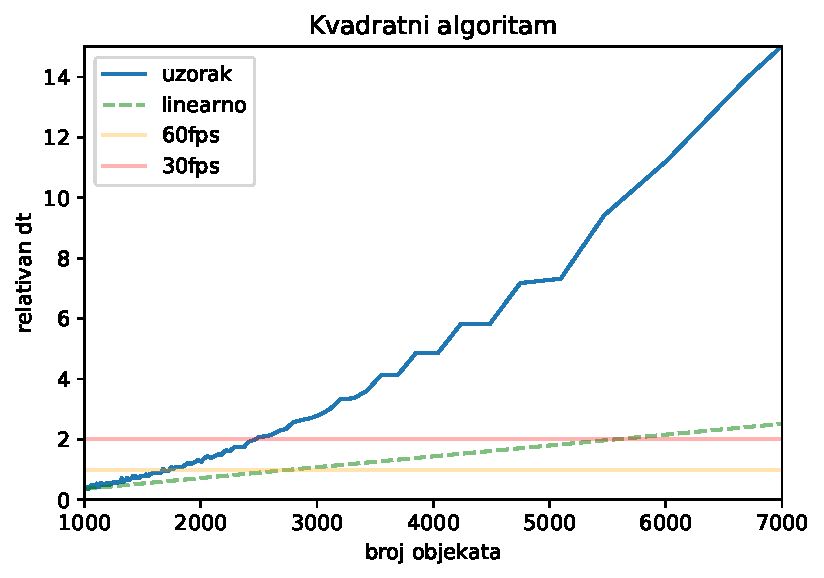
\includegraphics[
		trim= 0 0 0 19, clip,
		scale=1]{basicCollision.pdf}
	\caption{Relativan dt u zavisnosti od broja objekata - trivijalan algoritam.}
	\label{fig:basic} 
\end{figure}

\section{Oktri}

Na slici \ref{fig:oktri1} su prikazane performanse oktrija sa maksimalnom dubinom od deset nivoa i četri maksimalna elementa u listu pre podele na podoktante.
Prati referentnu liniju linearne zavisnosti na početku. 
I za manji broj objekata je višestruko bolji u odnosu na prethodno prikazani, pada ispod 60fps tek nakon 12 000 objekata, i ispod 30fps nakon 20 000.
Ipak, na slici \ref{fig:oktri2} se primećuje brže udaljavanje od linearne prave, što je za očekivati pošto algoriam nije linearne vremenske složenosti.

\begin{figure}[h!]
	\centerfloat
	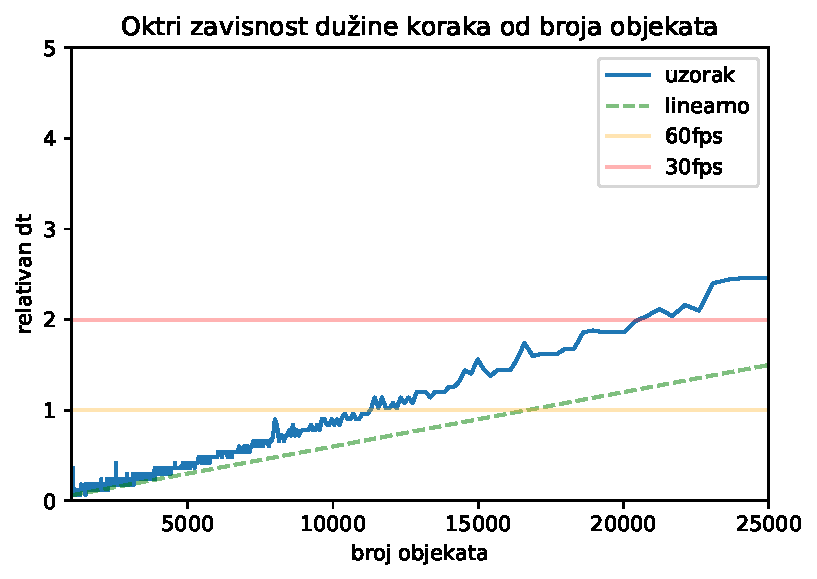
\includegraphics[
		trim=0 0 0 19,clip,
		scale=1]{oktri_dt_vs_numobj.pdf}
	\caption{Zavisnost relativnog dt od broja objekata - oktri.}
	\label{fig:oktri1}
\end{figure}

\begin{figure}[h!]
	\centerfloat
	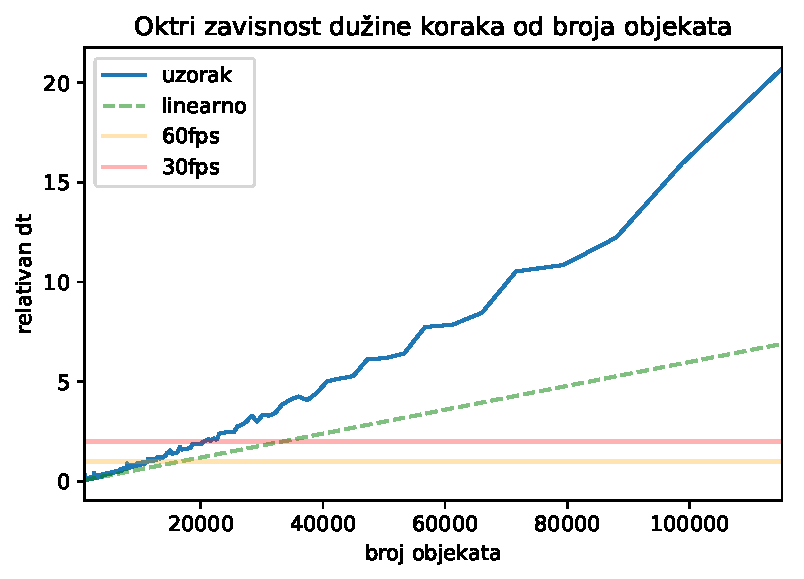
\includegraphics[
		trim=0 0 0 19,clip,
		scale=1]{oktri_dt_vs_numobj_zoomout.pdf}
	\caption{Zavisnost relativnog dt od broja objekata - oktri, više objekata.}
	\label{fig:oktri2}
\end{figure}

Oktri sa i bez duplikata su često sličnih performansi. Jedan primer kada je razlika ogromna je kada je veliki broj objekata na istom mestu.
Za potrebe demonstriranja se koristi scenario gde se objekti nasumično kreću i onda svi bivaju povučeni ka jednoj istoj tački.
Tada se svi nalaze na istom mestu za trenutak, i potom se razilaze.
Na slici \ref{fig:octreSpike} se vide tri manja plava skoka za oktri bez duplikata, i dva narandžasta skoka reda veličine za oktri sa duplikatima.
Za ovo merenje je isključeno razrešenje kolizije da bi više objekata bilo u koliziji, što pokazuje interesantno svojstvo da iako je potrebna dodatna obrada za razrešenje kolizije, 
ona onemogućava grupisanje preseka objekata i time ubrzava izvršavanje oktrija (i mnogih drugih algoritama detekcije kolizije).


\begin{figure}[h!]
	\centerfloat
	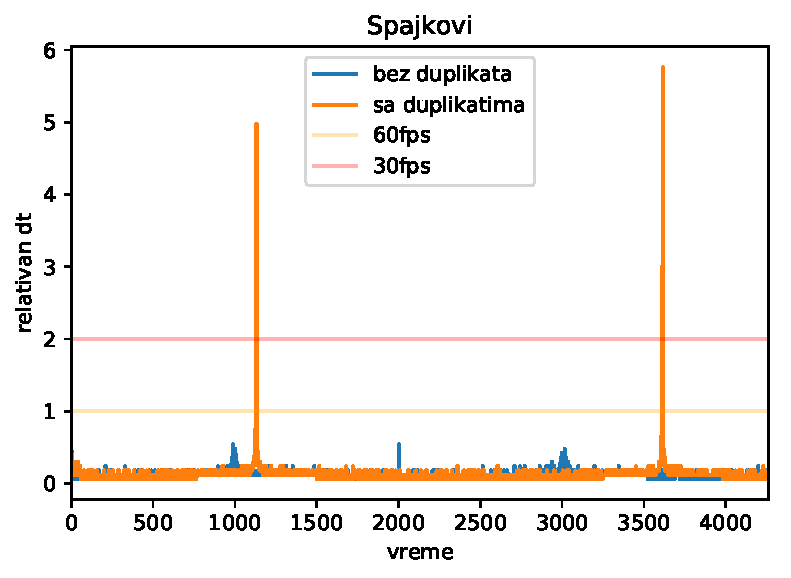
\includegraphics[
		trim=0 0 0 19,clip,
		scale=1]{octreeSpikes.pdf}
	\caption{Usporenje oktrija pri klasterovanju objekata.}
	\label{fig:octreSpike}
\end{figure}


Dok se razvijao projekat odabrana je konstanta 4 za maksimalan broj elemenata u listu oktrija proizvoljno, 
vodeći se logikom da je mali broj povoljan zbog izbegavanja kvadratnog broja upoređivanja, a da nije baš jedinica, kada bi se previše listovi delili.
Na slici \ref{fig:octree_leaf} se zapaža da četvorka nije loš izbor i tada je u proseku 69fps. 
Jedinica je najgori parametar pošto dovodi do viška rekurzivnog particionisanja prostora, relativan dt opada do koeficijenta 32 i nadalje naste.
Najbolja vrednost parametra je 32, kada je prosečno 94 što je čak 26.5\% bolje! 
Ubrzanje od 26.5\% je u praksi impresivno, pogotovo što je postignuto samo promenom jednog koeficijenta.
Pri merenju je fiskno 10 000 objekata i korišćen je oktri sa duplikatima.

\begin{figure}[h!]
	\centerfloat
	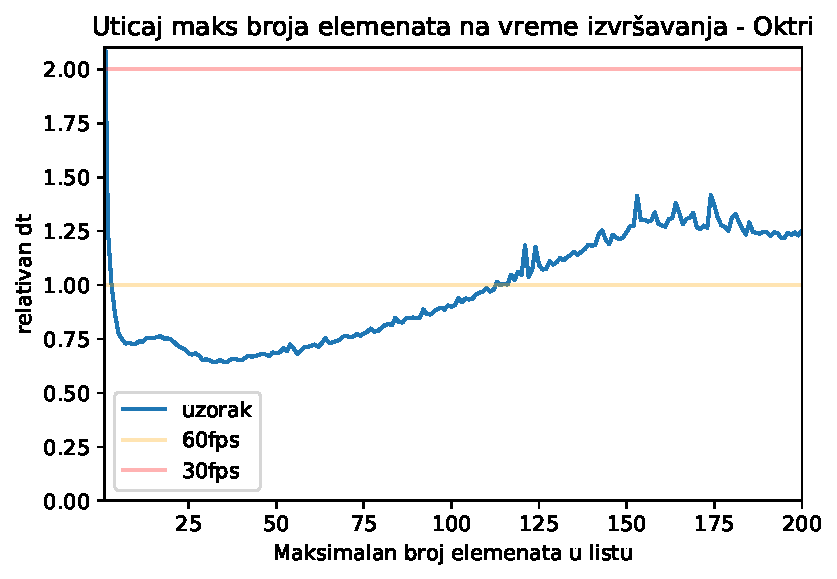
\includegraphics[
		trim=0 0 0 19,clip,
		scale=1]{octree_leaf.pdf}
	\caption{Relativan dt u zavisnosti od maksimalnog broja elemenata u listu oktrija}
	\label{fig:octree_leaf}
\end{figure}


Maksimalna dubina oktrija je postavljena na 10 tokom razvoja projekta. 
Njenom promenom se ne postiže mnogo, osim jakog usporenja kad bi se postavila na 1 ili 2, jer se tad skoro svi parovi moraju ispitati.
Vrednosti 9 do 12 predstavljaju razuman segment za odabir maksimalne dubine, jer omogućavaju dovoljno particionisanje prostora 
da se izbegne kvadratan broj operacija ispitivanja preseka,
a u slučaju da se više objekata preklapa će zaustaviti rano rekurzivne podele koje pokušavaju da ih podele u više oktanata.

\section{SAP}


SAP se ponaša dopustivo do 11 000 objekata, što se vidi na slici \ref{fig:sap1}.

\begin{figure}[h!]
	\centerfloat
	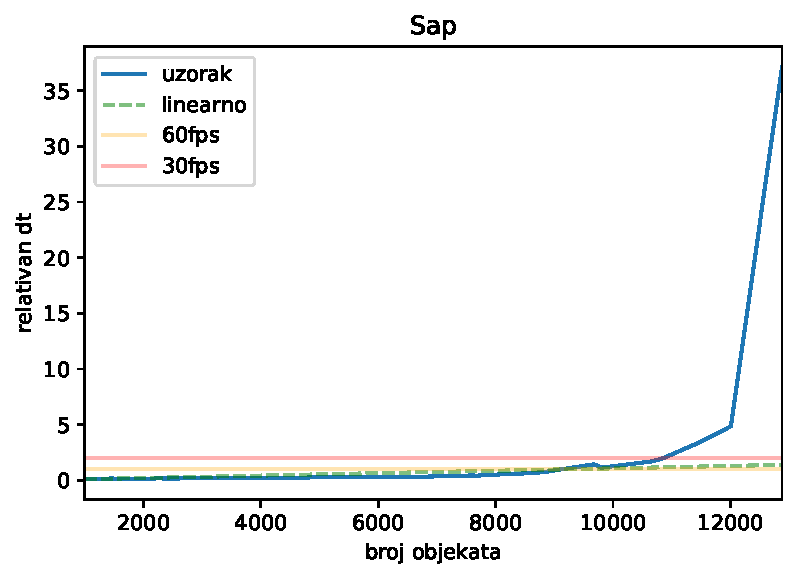
\includegraphics[
		trim=0 0 0 19,clip,
		scale=1]{sap1.pdf}
	\caption{Zavisnost relativnog dt od broja objekata - SAP.}
	\label{fig:sap1}
\end{figure}

Preko 11 000 objekata počinje da se manifestuje njegova glavna razlika u odnosu na ostale algoritme.
Za veći broj objekata potrebno je više vremena da se obradi detekcija kolizije, što produžava vreme između dva ažuriranja pozicija.
Što je vreme između dva ažuriranja pozicija veće, to je i više vremena proteklo u simulaciji, samim tim će i objekti biti udaljeniji od svojih prethodnih pozicija 
nego što bi bio slučaj sa kraćim vremenom između dva koraka. Veći pomeraj objekata znači da je niz koji se održava sortiranim u SAP algoritmu daleko od toga da bude 
sortiran, pa je potrebno dodatno zamena elemenata u nizu dok on ponovo postane sortiran. 
To opet povećava vreme izvršavanja između dva koraka, što vodi većoj udaljenosti objekta od prošle pozicije, i tako u krug.

Taj princip je prikazan na slici \ref{fig:dtSapCrawl}, gde je fiskno 12 800 objekata na sceni, a vreme izvršavanja eksplodira, čak ispod jednog iscrtavanja u sekundi.
Vidi se direktna veza broja zamena i relativnog dt pošto se zbog kvadratnog broja zamena katastrofalno uspori algoritam.

\begin{figure}[h!]
	\centerfloat
	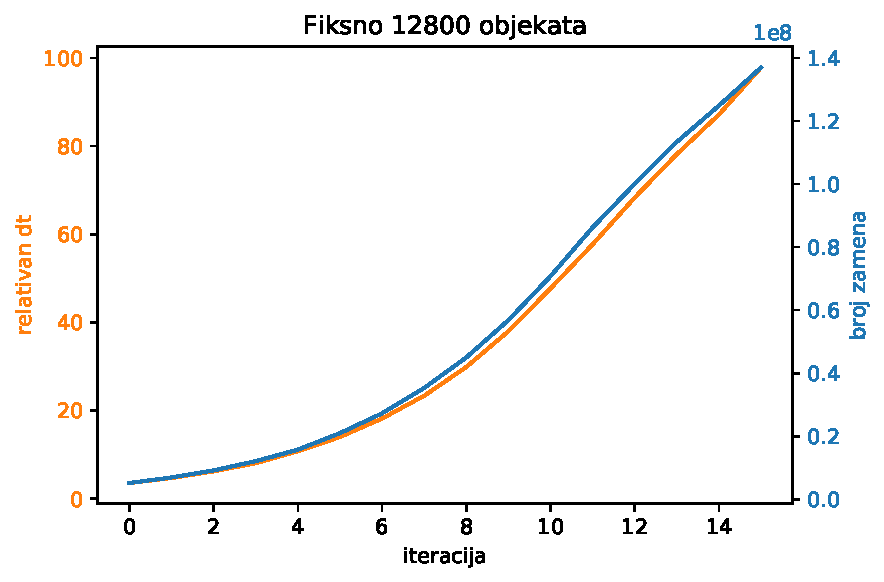
\includegraphics[
		trim=0 0 0 19,clip,
		scale=1]{dtSapCrawl.pdf}
	\caption{SAP: povratna sprega povećava dt, iako je fiksan broj objekata.}
	\label{fig:dtSapCrawl}
\end{figure}

Osim što brzina kretanja može katastrofalno da utiče na performanse SAP algoritma, tako i smanjivanje brzine utiče povoljno na njegovo vreme izvršavanja.
Upoređivanje vremena za tri različite brzine objekata je dato na slici \ref{fig:sap3speeds}. 
Prvi je meren pri podrazumevanoj brzini, drugi pri duplo manjoj i treći pri četri puta manjoj brzini.
Što se sporije objekti kreću to je tačka kada počinje povratna sprega da uzima maha više odložena.
U svakom slučaju će se to desiti nakon nekog broja elemenata, tako da u zavisnosti od situacije SAP algoritam može biti loš ili idealan.

\begin{figure}[h!]
	\centerfloat
	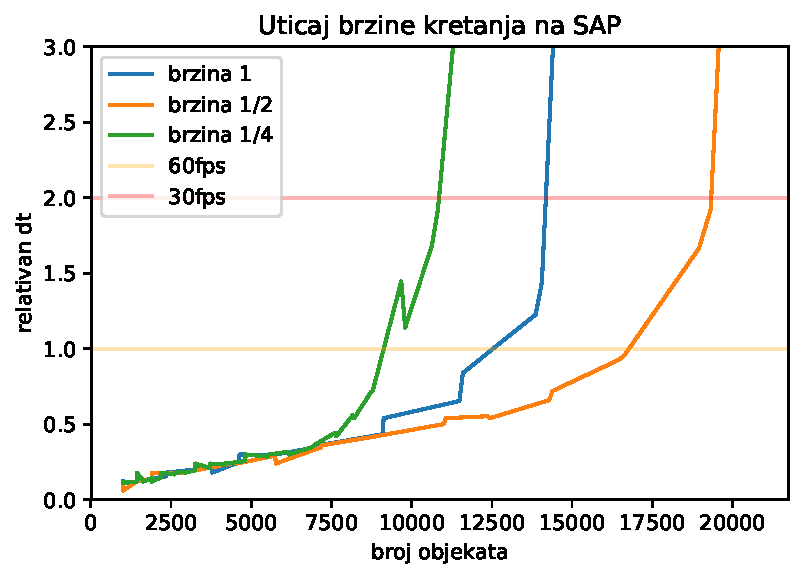
\includegraphics[
		trim=0 0 0 19,clip,
		scale=1]{sap3speeds.pdf}
	\caption{Upoređivanje rasta relativnog dt u zavisnosti od objekta pri njihovim različitim brzinama - SAP.}
	\label{fig:sap3speeds}
\end{figure}

U do sada razmatranim slučajevima svi prelaze granicu od dva relativna dt pre 20 000 objekata.
Na slici \ref{fig:sap_great} je prikazana situacija kada je SAP algoritam ubedljivo najbolji.
Prilikom merenja je isključeno iscrtavanje pošto ono traje duže od samog algoritma kolizije u ovakvom slučaju,
što se može videti na \ref{fig:drawVsNoDraw}, jer na oko 50 000 objekata relativan dt prelazi 2.
Ovde je išestruko je bolji SAP od ostalih, dostižući 60fps tek na 75 000, a 30fps na 92 000 objekata.
Pritom ostaje ispod referentne linearne prave, sve do kraja kada se približava broju objekata koji vodi 
do akumuliranja usporavanja, što je oko 100 000.


\begin{figure}[h!]
	\centerfloat
	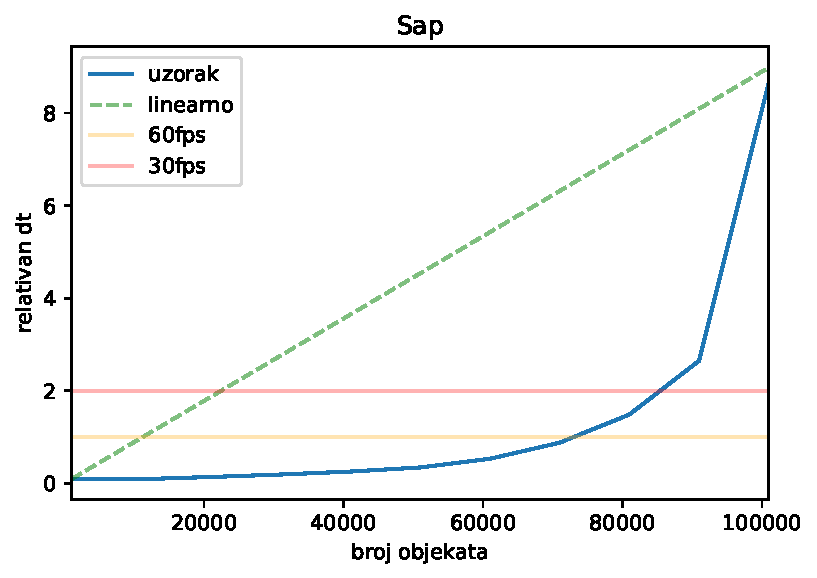
\includegraphics[
		trim=0 0 0 19,clip,
		scale=1]{sap_great.pdf}
	\caption{Relativan dt u zavisnosti od objekta kada se sporo kreću - SAP.}
	\label{fig:sap_great}
\end{figure}


% ==============================================================================
\chapter{Zaključak}
\label{sec:zakljucak}
% ==============================================================================

Zaključak... 


% ------------------------------------------------------------------------------
% Literatura
% ------------------------------------------------------------------------------
\literatura

% ==============================================================================
% Završni deo teze i prilozi
\backmatter
% ==============================================================================


% \appendix
% \section{Dodatak}
% Dodatak.

\end{document}
